\chapter{Programming with Python}\label{s:python}

The best way to learn how to program is to do something useful, so this
introduction to Python is built around a common scientific task: data
analysis.

Our real goal isn't to teach you Python, but to teach you the basic
concepts that all programming depends on. We use Python in our lessons
because:

\begin{swcenumerate}
\item
  we have to use \emph{something} for examples;
\item
  it's free, well-documented, and runs almost everywhere;
\item
  it has a large (and growing) user base among scientists; and
\item
  experience shows that it's easier for novices to pick up than most
  other languages.
\end{swcenumerate}

But the two most important things are to use whatever language your
colleagues are using, so that you can share you work with them easily,
and to use that language \emph{well}.

\section{Analyzing Patient Data}

We are studying inflammation in patients who have been given a new
treatment for arthritis, and need to analyze the first dozen data sets.
The data sets are stored in \gl{comma-separated values}{g:csv}
(CSV) format: each row holds information for a single patient, and the
columns represent successive days. The first few rows of our first file
look like this:

\begin{VerbFile}
0,0,1,3,1,2,4,7,8,3,3,3,10,5,7,4,7,7,12,18,6,13,11,11,7,7,4,6,8,8,4,4,5,7,3,4,2,3,0,0
0,1,2,1,2,1,3,2,2,6,10,11,5,9,4,4,7,16,8,6,18,4,12,5,12,7,11,5,11,3,3,5,4,4,5,5,1,1,0,1
0,1,1,3,3,2,6,2,5,9,5,7,4,5,4,15,5,11,9,10,19,14,12,17,7,12,11,7,4,2,10,5,4,2,2,3,2,2,1,1
0,0,2,0,4,2,2,1,6,7,10,7,9,13,8,8,15,10,10,7,17,4,4,7,6,15,6,4,9,11,3,5,6,3,3,4,2,3,2,1
0,1,1,3,3,1,3,5,2,4,4,7,6,5,3,10,8,10,6,17,9,14,9,7,13,9,12,6,7,7,9,6,3,2,2,4,2,0,1,1
\end{VerbFile}

We want to:

\begin{swcitemize}
\item
  load that data into memory,
\item
  calculate the average inflammation per day across all patients, and
\item
  plot the result.
\end{swcitemize}

To do all that, we'll have to learn a little bit about programming.

\begin{objectives}
\begin{swcitemize}
\item
  Explain what a library is, and what libraries are used for.
\item
  Load a Python library and use the things it contains.
\item
  Read tabular data from a file into a program.
\item
  Assign values to variables.
\item
  Select individual values and subsections from data.
\item
  Perform operations on arrays of data.
\item
  Display simple graphs.
\end{swcitemize}
\end{objectives}

\subsection{Loading Data}

Words are useful, but what's more useful are the sentences and stories
we use them to build. Similarly, while a lot of powerful tools are built
into languages like Python, even more lives in the
\gl{libraries}{g:library} they are used to build.

In order to load our inflammation data, we need to
\gl{import}{g:import} a library called NumPy that knows how to
operate on matrices:

\begin{VerbIn}
import numpy
\end{VerbIn}

Importing a library is like getting a piece of lab equipment out of a
storage locker and setting it up on the bench. Once it's done, we can
ask the library to read our data file for us:

\begin{VerbIn}
numpy.loadtxt(fname='inflammation-01.csv', delimiter=',')
\end{VerbIn}

\begin{VerbOut}
array([[ 0.,  0.,  1., ...,  3.,  0.,  0.],
       [ 0.,  1.,  2., ...,  1.,  0.,  1.],
       [ 0.,  1.,  1., ...,  2.,  1.,  1.],
       ...,
       [ 0.,  1.,  1., ...,  1.,  1.,  1.],
       [ 0.,  0.,  0., ...,  0.,  2.,  0.],
       [ 0.,  0.,  1., ...,  1.,  1.,  0.]])
\end{VerbOut}

The expression \texttt{numpy.loadtxt(...)} is a
\gl{function call}{g:function-call} that asks Python to run the
function \texttt{loadtxt} that belongs to the \texttt{numpy} library.
This \gl{dotted notation}{g:dotted-notation} is used everywhere in
Python to refer to the parts of things as \texttt{whole.part}.

\texttt{numpy.loadtxt} has two \gl{parameters}{g:parameter}: the
name of the file we want to read, and the
\gl{delimiter}{g:delimiter} that separates values on a line. These
both need to be character strings (or \gl{strings}{g:string} for
short), so we put them in quotes.

When we are finished typing and press Shift+Enter, the notebook runs our
command. Since we haven't told it to do anything else with the
function's output, the notebook displays it. In this case, that output
is the data we just loaded. By default, only a few rows and columns are
shown (with \texttt{...} to omit elements when displaying big arrays).
To save space, Python displays numbers as \texttt{1.} instead of
\texttt{1.0} when there's nothing interesting after the decimal point.

Our call to \texttt{numpy.loadtxt} read our file, but didn't save the
data in memory. To do that, we need to \gl{assign}{g:assignment}
the array to a \gl{variable}{g:variable}. A variable is just a
name for a value, such as \texttt{x}, \texttt{current\_temperature}, or
\texttt{subject\_id}. We can create a new variable simply by assigning a
value to it using \texttt{=}:

\begin{VerbIn}
weight_kg = 55
\end{VerbIn}

Once a variable has a value, we can print it:

\begin{VerbIn}
print weight_kg
\end{VerbIn}

\begin{VerbOut}
55
\end{VerbOut}

and do arithmetic with it:

\begin{VerbIn}
print 'weight in pounds:', 2.2 * weight_kg
\end{VerbIn}

\begin{VerbOut}
weight in pounds: 121.0
\end{VerbOut}

We can also change a variable's value by assigning it a new one:

\begin{VerbIn}
weight_kg = 57.5
print 'weight in kilograms is now:', weight_kg
\end{VerbIn}

\begin{VerbOut}
weight in kilograms is now: 57.5
\end{VerbOut}

As the example above shows, we can print several things at once by
separating them with commas.

If we imagine the variable as a sticky note with a name written on it,
assignment is like putting the sticky note on a particular value (\figref{f:assignment}).

\swcgraphics{f:assignment}{Assignment}{novice/python/img/python-sticky-note-variables-01.pdf}{0.75}

This means that assigning a value to one variable does \emph{not} change
the values of other variables. For example, let's store the subject's
weight in pounds in a variable (\figref{f:before-changing-weight}):

\begin{VerbIn}
weight_lb = 2.2 * weight_kg
print 'weight in kilograms:', weight_kg, 'and in pounds:', weight_lb
\end{VerbIn}

\begin{VerbOut}
weight in kilograms: 57.5 and in pounds: 126.5
\end{VerbOut}

\swcgraphics{f:before-changing-weight}{Before Changing Weight}{novice/python/img/python-sticky-note-variables-02.pdf}{0.75}

and then change \texttt{weight\_kg} (\figref{f:after-changing-weight}):

\begin{VerbIn}
weight_kg = 100.0
print 'weight in kilograms is now:', weight_kg, 'and weight in pounds is still:', weight_lb
\end{VerbIn}

\begin{VerbOut}
weight in kilograms is now: 100.0 and weight in pounds is still: 126.5
\end{VerbOut}

\swcgraphics{f:after-changing-weight}{After Changing Weight}{novice/python/img/python-sticky-note-variables-03.pdf}{0.75}

Since \texttt{weight\_lb} doesn't ``remember'' where its value came
from, it isn't automatically updated when \texttt{weight\_kg} changes.
This is different from the way spreadsheets work.

Now that we know how to assign things to variables, let's re-run
\texttt{numpy.loadtxt} and save its result:

\begin{VerbIn}
data = numpy.loadtxt(fname='inflammation-01.csv', delimiter=',')
\end{VerbIn}

This statement doesn't produce any output because assignment doesn't
display anything. If we want to check that our data has been loaded, we
can print the variable's value:

\begin{VerbIn}
print data
\end{VerbIn}

\begin{VerbOut}
[[ 0.  0.  1. ...,  3.  0.  0.]
 [ 0.  1.  2. ...,  1.  0.  1.]
 [ 0.  1.  1. ...,  2.  1.  1.]
 ...,
 [ 0.  1.  1. ...,  1.  1.  1.]
 [ 0.  0.  0. ...,  0.  2.  0.]
 [ 0.  0.  1. ...,  1.  1.  0.]]
\end{VerbOut}

\begin{challenge}
  Draw diagrams showing what variables refer to what values after each
  statement in the following program:

\begin{VerbIn}
mass = 47.5
age = 122
mass = mass * 2.0
age = age - 20
\end{VerbIn}
\end{challenge}

\begin{challenge}
  What does the following program print out?
\begin{VerbIn}
first, second = `Grace', `Hopper'
third, fourth = second, first
print third, fourth
\end{VerbIn}
\end{challenge}

\subsection{Manipulating Data}

Now that our data is in memory, we can start doing things with it.
First, let's ask what \gl{type}{g:data-type} of thing
\texttt{data} refers to:

\begin{VerbIn}
print type(data)
\end{VerbIn}

\begin{VerbOut}
<type 'numpy.ndarray'>
\end{VerbOut}

The output tells us that \texttt{data} currently refers to an
N-dimensional array created by the NumPy library. We can see what its
\gl{shape}{g:shape} is like this:

\begin{VerbIn}
print data.shape
\end{VerbIn}

\begin{VerbOut}
(60, 40)
\end{VerbOut}

This tells us that \texttt{data} has 60 rows and 40 columns.
\texttt{data.shape} is a \gl{member}{g:member} of \texttt{data},
i.e., a value that is stored as part of a larger value. We use the same
dotted notation for the members of values that we use for the functions
in libraries because they have the same part-and-whole relationship.

If we want to get a single value from the matrix, we must provide an
\gl{index}{g:index} in square brackets, just as we do in math:

\begin{VerbIn}
print 'first value in data:', data[0, 0]
\end{VerbIn}

\begin{VerbOut}
first value in data: 0.0
\end{VerbOut}

\begin{VerbIn}
print 'middle value in data:', data[30, 20]
\end{VerbIn}

\begin{VerbOut}
middle value in data: 13.0
\end{VerbOut}

The expression \texttt{data{[}30, 20{]}} may not surprise you, but
\texttt{data{[}0, 0{]}} might. Programming languages like Fortran and
MATLAB start counting at 1, because that's what human beings have done
for thousands of years. Languages in the C family (including C++, Java,
Perl, and Python) count from 0 because that's simpler for computers to
do. As a result, if we have an M×N array in Python, its indices go from
0 to M-1 on the first axis and 0 to N-1 on the second. It takes a bit of
getting used to, but one way to remember the rule is that the index is
how many steps we have to take from the start to get the item we want.

\begin{swcbox}{In the Corner}

What may also surprise you is that when Python displays an array, it
shows the element with index \texttt{{[}0, 0{]}} in the upper left
corner rather than the lower left. This is consistent with the way
mathematicians draw matrices, but different from the Cartesian
coordinates. The indices are (row, column) instead of (column, row) for
the same reason.

\end{swcbox}

An index like \texttt{{[}30, 20{]}} selects a single element of an
array, but we can select whole sections as well. For example, we can
select the first ten days (columns) of values for the first four (rows)
patients like this:

\begin{VerbIn}
print data[0:4, 0:10]
\end{VerbIn}

\begin{VerbOut}
[[ 0.  0.  1.  3.  1.  2.  4.  7.  8.  3.]
 [ 0.  1.  2.  1.  2.  1.  3.  2.  2.  6.]
 [ 0.  1.  1.  3.  3.  2.  6.  2.  5.  9.]
 [ 0.  0.  2.  0.  4.  2.  2.  1.  6.  7.]]
\end{VerbOut}

The \gl{slice}{g:slice} \texttt{0:4} means, ``Start at index 0 and
go up to, but not including, index 4.'' Again, the
up-to-but-not-including takes a bit of getting used to, but the rule is
that the difference between the upper and lower bounds is the number of
values in the slice.

We don't have to start slices at 0:

\begin{VerbIn}
print data[5:10, 0:10]
\end{VerbIn}

\begin{VerbOut}
[[ 0.  0.  1.  2.  2.  4.  2.  1.  6.  4.]
 [ 0.  0.  2.  2.  4.  2.  2.  5.  5.  8.]
 [ 0.  0.  1.  2.  3.  1.  2.  3.  5.  3.]
 [ 0.  0.  0.  3.  1.  5.  6.  5.  5.  8.]
 [ 0.  1.  1.  2.  1.  3.  5.  3.  5.  8.]]
\end{VerbOut}

and we don't have to take all the values in the slice---if we provide a
\gl{stride}{g:stride}, Python takes values spaced that far apart:

\begin{VerbIn}
print data[0:10:3, 0:10:2]
\end{VerbIn}

\begin{VerbOut}
[[ 0.  1.  1.  4.  8.]
 [ 0.  2.  4.  2.  6.]
 [ 0.  2.  4.  2.  5.]
 [ 0.  1.  1.  5.  5.]]
\end{VerbOut}

Here, we have taken rows 0, 3, 6, and 9, and columns 0, 2, 4, 6, and 8.
(Again, we always include the lower bound, but stop when we reach or
cross the upper bound.)

We also don't have to include the upper and lower bound on the slice. If
we don't include the lower bound, Python uses 0 by default; if we don't
include the upper, the slice runs to the end of the axis, and if we
don't include either (i.e., if we just use `:' on its own), the slice
includes everything:

\begin{VerbIn}
small = data[:3, 36:]
print 'small is:'
print small
\end{VerbIn}

\begin{VerbOut}
small is:
[[ 2.  3.  0.  0.]
 [ 1.  1.  0.  1.]
 [ 2.  2.  1.  1.]]
\end{VerbOut}

Arrays also know how to perform common mathematical operations on their
values. If we want to find the average inflammation for all patients on
all days, for example, we can just ask the array for its mean value

\begin{VerbIn}
print data.mean()
\end{VerbIn}

\begin{VerbOut}
6.14875
\end{VerbOut}

\texttt{mean} is a \gl{method}{g:method} of the array, i.e., a
function that belongs to it in the same way that the member
\texttt{shape} does. If variables are nouns, methods are verbs: they are
what the thing in question knows how to do. This is why
\texttt{data.shape} doesn't need to be called (it's just a thing) but
\texttt{data.mean()} does (it's an action). It is also why we need empty
parentheses for \texttt{data.mean()}: even when we're not passing in any
parameters, parentheses are how we tell Python to go and do something
for us.

NumPy arrays have lots of useful methods:

\begin{VerbIn}
print 'maximum inflammation:', data.max()
print 'minimum inflammation:', data.min()
print 'standard deviation:', data.std()
\end{VerbIn}

\begin{VerbOut}
maximum inflammation: 20.0
minimum inflammation: 0.0
standard deviation: 4.61383319712
\end{VerbOut}

When analyzing data, though, we often want to look at partial
statistics, such as the maximum value per patient or the average value
per day. One way to do this is to select the data we want to create a
new temporary array, then ask it to do the calculation:

\begin{VerbIn}
patient_0 = data[0, :] # 0 on the first axis, everything on the second
print 'maximum inflammation for patient 0:', patient_0.max()
\end{VerbIn}

\begin{VerbOut}
maximum inflammation for patient 0: 18.0
\end{VerbOut}

We don't actually need to store the row in a variable of its own.
Instead, we can combine the selection and the method call:

\begin{VerbIn}
print 'maximum inflammation for patient 2:', data[2, :].max()
\end{VerbIn}

\begin{VerbOut}
maximum inflammation for patient 2: 19.0
\end{VerbOut}

\swcgraphics{f:across-axis}{Operating Across an Axis}{novice/python/img/python-operations-across-axes.pdf}{0.75}

What if we need the maximum inflammation for \emph{all} patients, or the
average for each day? As \figref{f:across-axis} shows, we want to perform the
operation across an axis.
To support this, most array methods allow us to specify the axis we want
to work on. If we ask for the average across axis 0, we get:

\begin{VerbIn}
print data.mean(axis=0)
\end{VerbIn}

\begin{VerbOut}
[  0.           0.45         1.11666667   1.75         2.43333333   3.15
   3.8          3.88333333   5.23333333   5.51666667   5.95         5.9
   8.35         7.73333333   8.36666667   9.5          9.58333333
  10.63333333  11.56666667  12.35        13.25        11.96666667
  11.03333333  10.16666667  10.           8.66666667   9.15         7.25
   7.33333333   6.58333333   6.06666667   5.95         5.11666667   3.6
   3.3          3.56666667   2.48333333   1.5          1.13333333
   0.56666667]
\end{VerbOut}

As a quick check, we can ask this array what its shape is:

\begin{VerbIn}
print data.mean(axis=0).shape
\end{VerbIn}

\begin{VerbOut}
(40,)
\end{VerbOut}

The expression \texttt{(40,)} tells us we have an N×1 vector, so this is
the average inflammation per day for all patients. If we average across
axis 1, we get:

\begin{VerbIn}
print data.mean(axis=1)
\end{VerbIn}

\begin{VerbOut}
[ 5.45   5.425  6.1    5.9    5.55   6.225  5.975  6.65   6.625  6.525
  6.775  5.8    6.225  5.75   5.225  6.3    6.55   5.7    5.85   6.55
  5.775  5.825  6.175  6.1    5.8    6.425  6.05   6.025  6.175  6.55
  6.175  6.35   6.725  6.125  7.075  5.725  5.925  6.15   6.075  5.75
  5.975  5.725  6.3    5.9    6.75   5.925  7.225  6.15   5.95   6.275  5.7
  6.1    6.825  5.975  6.725  5.7    6.25   6.4    7.05   5.9  ]
\end{VerbOut}

which is the average inflammation per patient across all days.

\begin{swcbox}{Slicing}
A subsection of an array is called a \gl{slice}{g:slice}. We can
take slices of character strings as well:

\begin{VerbIn}
element = 'oxygen'
print 'first three characters:', element[0:3]
print 'last three characters:', element[3:6]
\end{VerbIn}

\begin{VerbOut}
first three characters: oxy
last three characters: gen
\end{VerbOut}
\end{swcbox}

\begin{challenge}
  What is the value of \texttt{element{[}:4{]}}? What about
  \texttt{element{[}4:{]}}? Or \texttt{element{[}:{]}}?
\end{challenge}

\begin{challenge}
  What is \texttt{element{[}-1{]}}? What is \texttt{element{[}-2{]}}?
  Given those answers, explain what \texttt{element{[}1:-1{]}} does.
\end{challenge}

\begin{challenge}
  The expression \texttt{element{[}3:3{]}} produces an
  \gl{empty string}{g:empty-string}, i.e., a string that contains
  no characters. If \texttt{data} holds our array of patient data, what
  does \texttt{data{[}3:3, 4:4{]}} produce? What about
  \texttt{data{[}3:3, :{]}}?
\end{challenge}

\subsection{Plotting}

The mathematician Richard Hamming once said, ``The purpose of computing
is insight, not numbers,'' and the best way to develop insight is often
to visualize data. Visualization deserves an entire lecture (or course)
of its own, but we can explore a few features of Python's
\texttt{matplotlib} here. First, let's tell the IPython Notebook that we
want our plots displayed inline, rather than in a separate viewing
window:

\begin{VerbIn}
%matplotlib inline
\end{VerbIn}

The \texttt{\%} at the start of the line signals that this is a
command for the notebook, rather than a statement in Python. Next, we
will import the \texttt{pyplot} module from \texttt{matplotlib} and
use two of its functions to create and display a heat map of our data
(\figref{f:initial-heatmap}):

\begin{VerbIn}
from matplotlib import pyplot
pyplot.imshow(data)
pyplot.show()
\end{VerbIn}

\swcgraphics{f:initial-heatmap}{Heat Map of Inflammation Data}{novice/python/img/initial-heatmap.png}{1.0}

Blue regions in this heat map are low values, while red shows high
values. As we can see, inflammation rises and falls over a 40-day
period. Let's take a look at the average inflammation over time (\figref{f:ave-inflammation}):

\begin{VerbIn}
ave_inflammation = data.mean(axis=0)
pyplot.plot(ave_inflammation)
pyplot.show()
\end{VerbIn}

\swcgraphics{f:ave-inflammation}{Average Inflammation over Time}{novice/python/img/ave-inflammation.png}{0.5}

Here, we have put the average per day across all patients in the
variable \texttt{ave\_inflammation}, then asked \texttt{pyplot} to
create and display a line graph of those values. The result is roughly a
linear rise and fall, which is suspicious: based on other studies, we
expect a sharper rise and slower fall. Let's have a look at two other
statistics, the maximum (\figref{f:max-inflammation}) and minimum (\figref{f:min-inflammation}) per day:

\begin{VerbIn}
pyplot.plot(data.max(axis=0))
pyplot.show()

pyplot.plot(data.min(axis=0))
pyplot.show()
\end{VerbIn}

\swcgraphics{f:max-inflammation}{Maximum Inflammation per Day}{novice/python/img/max-inflammation.png}{0.5}

\swcgraphics{f:min-inflammation}{Minimum Inflammation per Day}{novice/python/img/min-inflammation.png}{0.5}

The maximum value rises and falls perfectly smoothly, while the minimum
seems to be a step function. Neither result seems particularly likely,
so either there's a mistake in our calculations or something is wrong
with our data.

\begin{challenge}
  Why do all of our plots stop just short of the upper end of our graph?
  Why are the vertical lines in our plot of the minimum inflammation per
  day not vertical?
\end{challenge}

\begin{challenge}
  Create a plot showing the standard deviation of the inflammation data
  for each day across all patients.
\end{challenge}

\subsection{Wrapping Up}

It's very common to create an \gl{alias}{g:alias-library} for a
library when importing it in order to reduce the amount of typing we
have to do. \figref{f:combined-inflammation} shows our three plots
side by side using aliases for \texttt{numpy} and \texttt{pyplot}:

\begin{VerbIn}
import numpy as np
from matplotlib import pyplot as plt

data = np.loadtxt(fname='inflammation-01.csv', delimiter=',')

plt.figure(figsize=(10.0, 3.0))

plt.subplot(1, 3, 1)
plt.ylabel('average')
plt.plot(data.mean(0))

plt.subplot(1, 3, 2)
plt.ylabel('max')
plt.plot(data.max(0))

plt.subplot(1, 3, 3)
plt.ylabel('min')
plt.plot(data.min(0))

plt.tight_layout()
plt.show()
\end{VerbIn}

\swcgraphics{f:combined-inflammation}{Inflammation Statistics vs.\ Time}{novice/python/img/combined-inflammation.png}{0.5}

The first two lines re-load our libraries as \texttt{np} and
\texttt{plt}, which are the aliases most Python programmers use. The
call to \texttt{loadtxt} reads our data, and the rest of the program
tells the plotting library how large we want the figure to be, that
we're creating three sub-plots, what to draw for each one, and that we
want a tight layout. (Perversely, if we leave out that call to
\texttt{plt.tight\_layout()}, the graphs will actually be squeezed
together more closely.)

\begin{challenge}
  Modify the program to display the three plots on top of one another
  instead of side by side.
\end{challenge}

\begin{keypoints}
\begin{swcitemize}
\item
  Import a library into a program using \texttt{import libraryname}.
\item
  Use the \texttt{numpy} library to work with arrays in Python.
\item
  Use \texttt{variable = value} to assign a value to a variable in order
  to record it in memory.
\item
  Variables are created on demand whenever a value is assigned to them.
\item
  Use \texttt{print something} to display the value of
  \texttt{something}.
\item
  The expression \texttt{array.shape} gives the shape of an array.
\item
  Use \texttt{array{[}x, y{]}} to select a single element from an array.
\item
  Array indices start at 0, not 1.
\item
  Use \texttt{low:high} to specify a slice that includes the indices
  from \texttt{low} to \texttt{high-1}.
\item
  All the indexing and slicing that works on arrays also works on
  strings.
\item
  Use \texttt{\# some kind of explanation} to add comments to programs.
\item
  Use \texttt{array.mean()}, \texttt{array.max()}, and
  \texttt{array.min()} to calculate simple statistics.
\item
  Use \texttt{array.mean(axis=0)} or \texttt{array.mean(axis=1)} to
  calculate statistics across the specified axis.
\item
  Use the \texttt{pyplot} library from \texttt{matplotlib} for creating
  simple visualizations.
\end{swcitemize}
\end{keypoints}

\section{Creating Functions}

If we only had one data set to analyze, it would probably be faster to
load the file into a spreadsheet and use that to plot some simple
statistics. But we have twelve files to check, and may have more in
future. In this lesson, we'll learn how to write a function so that we
can repeat several operations with a single command.

\begin{objectives}
\begin{swcitemize}
\item
  Define a function that takes parameters.
\item
  Return a value from a function.
\item
  Test and debug a function.
\item
  Explain what a call stack is, and trace changes to the call stack as
  functions are called.
\item
  Set default values for function parameters.
\item
  Explain why we should divide programs into small, single-purpose
  functions.
\end{swcitemize}
\end{objectives}

\subsection{Defining a Function}

Let's start by defining a function \texttt{fahr\_to\_kelvin} that
converts temperatures from Fahrenheit to Kelvin:

\begin{VerbIn}
def fahr_to_kelvin(temp):
    return ((temp - 32) * (5/9)) + 273.15
\end{VerbIn}

The definition opens with the word \texttt{def}, which is followed by
the name of the function and a parenthesized list of parameter names.
The \gl{body}{g:function-body} of the function---the statements
that are executed when it runs---is indented below the definition line,
typically by four spaces.

When we call the function, the values we pass to it are assigned to
those variables so that we can use them inside the function. Inside the
function, we use a \gl{return statement}{g:return-statement} to
send a result back to whoever asked for it.

Let's try running our function. Calling our own function is no different
from calling any other function:

\begin{VerbIn}
print 'freezing point of water:', fahr_to_kelvin(32)
print 'boiling point of water:', fahr_to_kelvin(212)
\end{VerbIn}

\begin{VerbOut}
freezing point of water: 273.15
boiling point of water: 273.15
\end{VerbOut}

We've successfully called the function that we defined, and we have
access to the value that we returned. Unfortunately, the value returned
doesn't look right. What went wrong?

\subsection{Debugging a Function}

\emph{Debugging} is when we fix a piece of code that we know is working
incorrectly. In this case, we know that \texttt{fahr\_to\_kelvin} is
giving us the wrong answer, so let's find out why.

For big pieces of code, there are tools called \emph{debuggers} that aid
in this process.

We just have a short function, so we'll debug by choosing some parameter
value, breaking our function into small parts, and printing out the
value of each part.

\begin{VerbIn}
# We'll use temp = 212, the boiling point of water, which was incorrect
print "212 - 32:", 212 - 32
\end{VerbIn}

\begin{VerbOut}
212 - 32: 180
\end{VerbOut}

\begin{VerbIn}
print "(212 - 32) * (5/9):", (212 - 32) * (5/9)
\end{VerbIn}

\begin{VerbOut}
(212 - 32) * (5/9): 0
\end{VerbOut}

Aha! The problem comes when we multiply by \texttt{5/9}. This is because
\texttt{5/9} is actually 0.

\begin{VerbIn}
5/9
\end{VerbIn}

\begin{VerbOut}
0
\end{VerbOut}

Computers store numbers in one of two ways: as
\gl{integers}{g:integer} or as \gl{floating-point
numbers}{g:float} (or floats). The first are the numbers we usually count with;
the second have fractional parts. Addition, subtraction and
multiplication work on both as we'd expect, but division works
differently. If we divide one integer by another, we get the quotient
without the remainder:

\begin{VerbIn}
print '10/3 is:', 10/3
\end{VerbIn}

\begin{VerbOut}
10/3 is: 3
\end{VerbOut}

If either part of the division is a float, on the other hand, the
computer creates a floating-point answer:

\begin{VerbIn}
print '10.0/3 is:', 10.0/3
\end{VerbIn}

\begin{VerbOut}
10.0/3 is: 3.33333333333
\end{VerbOut}

The computer does this for historical reasons: integer operations were
much faster on early machines, and this behavior is actually useful in a
lot of situations. It's still confusing, though, so Python 3 produces a
floating-point answer when dividing integers if it needs to. We're still
using Python 2.7 in this class, though, so if we want \texttt{5/9} to
give us the right answer, we have to write it as \texttt{5.0/9},
\texttt{5/9.0}, or some other variation.

Let's fix our \texttt{fahr\_to\_kelvin} function with this new
knowledge.

\begin{VerbIn}
def fahr_to_kelvin(temp):
    return ((temp - 32) * (5.0/9.0)) + 273.15

print 'freezing point of water:', fahr_to_kelvin(32)
print 'boiling point of water:', fahr_to_kelvin(212)
\end{VerbIn}

\begin{VerbOut}
freezing point of water: 273.15
boiling point of water: 373.15
\end{VerbOut}

It works!

\subsection{Composing Functions}

Now that we've seen how to turn Fahrenheit into Kelvin, it's easy to
turn Kelvin into Celsius:

\begin{VerbIn}
def kelvin_to_celsius(temp):
    return temp - 273.15

print 'absolute zero in Celsius:', kelvin_to_celsius(0.0)
\end{VerbIn}

\begin{VerbOut}
absolute zero in Celsius: -273.15
\end{VerbOut}

What about converting Fahrenheit to Celsius? We could write out the
formula, but we don't need to. Instead, we can
\gl{compose}{g:function-composition} the two functions we have
already created:

\begin{VerbIn}
def fahr_to_celsius(temp):
    temp_k = fahr_to_kelvin(temp)
    result = kelvin_to_celsius(temp_k)
    return result

print 'freezing point of water in Celsius:', fahr_to_celsius(32.0)
\end{VerbIn}

\begin{VerbOut}
freezing point of water in Celsius: 0.0
\end{VerbOut}

This is our first taste of how larger programs are built: we define
basic operations, then combine them in ever-large chunks to get the
effect we want. Real-life functions will usually be larger than the ones
shown here---typically half a dozen to a few dozen lines---but they
shouldn't ever be much longer than that, or the next person who reads it
won't be able to understand what's going on.

\begin{challenge}
  ``Adding'' two strings produces their concatention: \texttt{'a' + 'b'}
  is \texttt{'ab'}. Write a function called \texttt{fence} that takes
  two parameters called \texttt{original} and \texttt{wrapper} and
  returns a new string that has the wrapper character at the beginning
  and end of the original:

\begin{VerbIn}
print fence('name', '*')
\end{VerbIn}

\begin{VerbOut}
*name*
\end{VerbOut}
\end{challenge}

\begin{challenge}
  If the variable \texttt{s} refers to a string, then \texttt{s{[}0{]}}
  is the string's first character and \texttt{s{[}-1{]}} is its last.
  Write a function called \texttt{outer} that returns a string made up
  of just the first and last characters of its input:

\begin{VerbIn}
print outer('helium')
\end{VerbIn}

\begin{VerbOut}
hm
\end{VerbOut}
\end{challenge}

\subsection{The Call Stack}

Let's take a closer look at what happens when we call
\texttt{fahr\_to\_celsius(32.0)}. To make things clearer, we'll start by
putting the initial value 32.0 in a variable and store the final result
in one as well:

\begin{VerbIn}
original = 32.0
final = fahr_to_celsius(original)
\end{VerbIn}

\swcgraphics{f:call-stack-01}{Initial Call Stack}{novice/python/img/python-call-stack-01.pdf}{0.75}

\figref{f:call-stack-01} shows what memory looks like after the first line has
been executed.

When we call \texttt{fahr\_to\_celsius}, Python \emph{doesn't} create
the variable \texttt{temp} right away. Instead, it creates something
called a \gl{stack frame}{g:stack-frame} to keep track of the
variables defined by \texttt{fahr\_to\_kelvin}. Initially, this stack
frame only holds the value of \texttt{temp} (\figref{f:call-stack-02}).

\swcgraphics{f:call-stack-02}{Call Stack Immediately Upon Call}{novice/python/img/python-call-stack-02.pdf}{0.75}

When we call \texttt{fahr\_to\_kelvin} inside
\texttt{fahr\_to\_celsius}, Python creates another stack frame to hold
\texttt{fahr\_to\_kelvin}'s variables (\figref{f:call-stack-03}).

\swcgraphics{f:call-stack-03}{Call Stack During Nested Function Call}{novice/python/img/python-call-stack-03.pdf}{0.75}

It does this because there are now two variables in play called
\texttt{temp}: the parameter to \texttt{fahr\_to\_celsius}, and the
parameter to \texttt{fahr\_to\_kelvin}. Having two variables with the
same name in the same part of the program would be ambiguous, so Python
(and every other modern programming language) creates a new stack frame
for each function call to keep that function's variables separate from
those defined by other functions.

When the call to \texttt{fahr\_to\_kelvin} returns a value, Python
throws away \texttt{fahr\_to\_kelvin}'s stack frame and creates a new
variable in the stack frame for \texttt{fahr\_to\_celsius} to hold the
temperature in Kelvin (\figref{f:call-stack-04}).

\swcgraphics{f:call-stack-04}{Call Stack Between Calls}{novice/python/img/python-call-stack-04.pdf}{0.75}

\swcgraphics{f:call-stack-05}{Call Stack During Second Call}{novice/python/img/python-call-stack-05.pdf}{0.75}

It then calls \texttt{kelvin\_to\_celsius}, which means it creates a
stack frame to hold that function's variables (\figref{f:call-stack-05}).
Once again, Python throws away that stack frame when
\texttt{kelvin\_to\_celsius} is done and creates the variable
\texttt{result} in the stack frame for \texttt{fahr\_to\_celsius}
(\figref{f:call-stack-06}).

\swcgraphics{f:call-stack-06}{Call Stack Immediately Before Final Return}{novice/python/img/python-call-stack-06.pdf}{0.75}

Finally, when \texttt{fahr\_to\_celsius} is done, Python throws away
\emph{its} stack frame and puts its result in a new variable called
\texttt{final} that lives in the stack frame we started with (\figref{f:call-stack-07}).

\swcgraphics{f:call-stack-07}{Call Stack After Calls Are Finished}{novice/python/img/python-call-stack-07.pdf}{0.75}

This final stack frame is always there; it holds the variables we
defined outside the functions in our code. What it \emph{doesn't} hold
is the variables that were in the various stack frames. If we try to get
the value of \texttt{temp} after our functions have finished running,
Python tells us that there's no such thing:

\begin{VerbIn}
print 'final value of temp after all function calls:', temp
\end{VerbIn}

\begin{VerbErr}
---------------------------------------------------------------------------
NameError                                 Traceback (most recent call last)
<ipython-input-12-ffd9b4dbd5f1> in <module>()
----> 1 print 'final value of temp after all function calls:', temp

NameError: name 'temp' is not definedfinal value of temp after all function calls:
\end{VerbErr}

Why go to all this trouble? Well, here's a function called \texttt{span}
that calculates the difference between the mininum and maximum values in
an array:

\begin{VerbIn}
import numpy

def span(a):
    diff = a.max() - a.min()
    return diff

data = numpy.loadtxt(fname='inflammation-01.csv', delimiter=',')
print 'span of data', span(data)
\end{VerbIn}

\begin{VerbOut}
 span of data 20.0
\end{VerbOut}

Notice that \texttt{span} assigns a value to a variable called
\texttt{diff}. We might very well use a variable with the same name to
hold data:

\begin{VerbIn}
diff = numpy.loadtxt(fname='inflammation-01.csv', delimiter=',')
print 'span of data:', span(diff)
\end{VerbIn}

\begin{VerbOut}
span of data: 20.0
\end{VerbOut}

We don't expect \texttt{diff} to have the value 20.0 after this function
call, so the name \texttt{diff} cannot refer to the same thing inside
\texttt{span} as it does in the main body of our program. And yes, we
could probably choose a different name than \texttt{diff} in our main
program in this case, but we don't want to have to read every line of
NumPy to see what variable names its functions use before calling any of
those functions, just in case they change the values of our variables.

The big idea here is \gl{encapsulation}{g:encapsulation}, and it's
the key to writing correct, comprehensible programs. A function's job is
to turn several operations into one so that we can think about a single
function call instead of a dozen or a hundred statements each time we
want to do something. That only works if functions don't interfere with
each other; if they do, we have to pay attention to the details once
again, which quickly overloads our short-term memory.

\begin{challenge}
  We previously wrote functions called \texttt{fence} and
  \texttt{outer}. Draw a diagram showing how the call stack changes when
  we run the following:
\begin{VerbIn}
print outer(fence('carbon', `+'))
\end{VerbIn}
\end{challenge}

\subsection{Testing and Documenting}

Once we start putting things in functions so that we can re-use them, we
need to start testing that those functions are working correctly. To see
how to do this, let's write a function to center a dataset around a
particular value:

\begin{VerbIn}
def center(data, desired):
    return (data - data.mean()) + desired
\end{VerbIn}

We could test this on our actual data, but since we don't know what the
values ought to be, it will be hard to tell if the result was correct.
Instead, let's use NumPy to create a matrix of 0's and then center that
around 3:

\begin{VerbIn}
z = numpy.zeros((2,2))
print center(z, 3)
\end{VerbIn}

\begin{VerbOut}
[[ 3.  3.]
 [ 3.  3.]]
\end{VerbOut}

That looks right, so let's try \texttt{center} on our real data:

\begin{VerbIn}
data = numpy.loadtxt(fname='inflammation-01.csv', delimiter=',')
print center(data, 0)
\end{VerbIn}

\begin{VerbOut}
[[-6.14875 -6.14875 -5.14875 ..., -3.14875 -6.14875 -6.14875]
 [-6.14875 -5.14875 -4.14875 ..., -5.14875 -6.14875 -5.14875]
 [-6.14875 -5.14875 -5.14875 ..., -4.14875 -5.14875 -5.14875]
 ...,
 [-6.14875 -5.14875 -5.14875 ..., -5.14875 -5.14875 -5.14875]
 [-6.14875 -6.14875 -6.14875 ..., -6.14875 -4.14875 -6.14875]
 [-6.14875 -6.14875 -5.14875 ..., -5.14875 -5.14875 -6.14875]]
\end{VerbOut}

It's hard to tell from the default output whether the result is correct,
but there are a few simple tests that will reassure us:

\begin{VerbIn}
print 'original min, mean, and max are:', data.min(), data.mean(), data.max()
centered = center(data, 0)
print 'min, mean, and and max of centered data are:', centered.min(), centered.mean(), centered.max()
\end{VerbIn}

\begin{VerbOut}
original min, mean, and max are: 0.0 6.14875 20.0
min, mean, and and max of centered data are: -6.14875 -3.49054118942e-15 13.85125
\end{VerbOut}

That seems almost right: the original mean was about 6.1, so the lower
bound from zero is how about -6.1. The mean of the centered data isn't
quite zero---we'll explore why not in the challenges---but it's pretty
close. We can even go further and check that the standard deviation
hasn't changed:

\begin{VerbIn}
print 'std dev before and after:', data.std(), centered.std()
\end{VerbIn}

\begin{VerbOut}
std dev before and after: 4.61383319712 4.61383319712
\end{VerbOut}

Those values look the same, but we probably wouldn't notice if they were
different in the sixth decimal place. Let's do this instead:

\begin{VerbIn}
print 'difference in standard deviations before and after:', data.std() - centered.std()
\end{VerbIn}

\begin{VerbOut}
difference in standard deviations before and after: -3.5527136788e-15
\end{VerbOut}

Again, the difference is very small. It's still possible that our
function is wrong, but it seems unlikely enough that we should probably
get back to doing our analysis. We have one more task first, though: we
should write some \gl{documentation}{g:documentation} for our
function to remind ourselves later what it's for and how to use it.

The usual way to put documentation in software is to add
\gl{comments}{g:comment} like this:

\begin{VerbIn}
# center(data, desired): return a new array containing the original data centered around the desired value.
def center(data, desired):
    return (data - data.mean()) + desired
\end{VerbIn}

There's a better way, though. If the first thing in a function is a
string that isn't assigned to a variable, that string is attached to the
function as its documentation:

\begin{VerbIn}
def center(data, desired):
    '''Return a new array containing the original data centered around the desired value.'''
    return (data - data.mean()) + desired
\end{VerbIn}

This is better because we can now ask Python's built-in help system to
show us the documentation for the function:

\begin{VerbIn}
help(center)
\end{VerbIn}

\begin{VerbOut}
Help on function center in module __main__:

center(data, desired)
    Return a new array containing the original data centered around the desired value.
\end{VerbOut}

A string like this is called a \gl{docstring}{g:docstring}. We
don't need to use triple quotes when we write one, but if we do, we can
break the string across multiple lines:

\begin{VerbIn}
def center(data, desired):
    '''Return a new array containing the original data centered around the desired value.
    Example: center([1, 2, 3], 0) => [-1, 0, 1]'''
    return (data - data.mean()) + desired

help(center)
\end{VerbIn}

\begin{VerbOut}
Help on function center in module __main__:

center(data, desired)
    Return a new array containing the original data centered around the desired value.
    Example: center([1, 2, 3], 0) => [-1, 0, 1]
\end{VerbOut}

\begin{challenge}
  Write a function called \texttt{analyze} that takes a filename as a
  parameter and displays the three graphs produced in the
  \urlfoot{01-numpy.ipynb}{previous lesson}, i.e.,
  \texttt{analyze('inflammation-01.csv')} should produce the graphs
  already shown, while \texttt{analyze('inflammation-02.csv')} should
  produce corresponding graphs for the second data set. Be sure to give
  your function a docstring.
\end{challenge}

\begin{challenge}
  Write a function \texttt{rescale} that takes an array as input and
  returns a corresponding array of values scaled to lie in the range 0.0
  to 1.0. (If \textbackslash{}(L\textbackslash{}) and
  \textbackslash{}(H\textbackslash{}) are the lowest and highest values
  in the original array, then the replacement for a value
  \textbackslash{}(v\textbackslash{}) should be \textbackslash{}((v-L) /
  (H-L)\textbackslash{}).) Be sure to give the function a docstring.
\end{challenge}

\begin{challenge}
  Run the commands \texttt{help(numpy.arange)} and
  \texttt{help(numpy.linspace)} to see how to use these functions to
  generate regularly-spaced values, then use those values to test your
  \texttt{rescale} function.
\end{challenge}

\subsection{Defining Defaults}

We have passed parameters to functions in two ways: directly, as in
\texttt{span(data)}, and by name, as in
\texttt{numpy.loadtxt(fname='something.csv', delimiter=',')}. In fact,
we can pass the filename to \texttt{loadtxt} without the
\texttt{fname=}:

\begin{VerbIn}
numpy.loadtxt('inflammation-01.csv', delimiter=',')
\end{VerbIn}

\begin{VerbOut}
array([[ 0.,  0.,  1., ...,  3.,  0.,  0.],
       [ 0.,  1.,  2., ...,  1.,  0.,  1.],
       [ 0.,  1.,  1., ...,  2.,  1.,  1.],
       ...,
       [ 0.,  1.,  1., ...,  1.,  1.,  1.],
       [ 0.,  0.,  0., ...,  0.,  2.,  0.],
       [ 0.,  0.,  1., ...,  1.,  1.,  0.]])
\end{VerbOut}

but we still need to say \texttt{delimiter=}:

\begin{VerbIn}
numpy.loadtxt('inflammation-01.csv', ',')
\end{VerbIn}

\begin{VerbErr}
---------------------------------------------------------------------------
TypeError                                 Traceback (most recent call last)
<ipython-input-26-e3bc6cf4fd6a> in <module>()
----> 1 numpy.loadtxt('inflammation-01.csv', ',')

/Users/gwilson/anaconda/lib/python2.7/site-packages/numpy/lib/npyio.pyc in loadtxt(fname, dtype, comments, delimiter, converters, skiprows, usecols, unpack, ndmin)
    775     try:
    776         # Make sure we're dealing with a proper dtype
--> 777         dtype = np.dtype(dtype)
    778         defconv = _getconv(dtype)
    779

TypeError: data type "," not understood
\end{VerbErr}

To understand what's going on, and make our own functions easier to use,
let's re-define our \texttt{center} function like this:

\begin{VerbIn}
def center(data, desired=0.0):
    '''Return a new array containing the original data centered around the desired value (0 by default).
    Example: center([1, 2, 3], 0) => [-1, 0, 1]'''
    return (data - data.mean()) + desired
\end{VerbIn}

The key change is that the second parameter is now written
\texttt{desired=0.0} instead of just \texttt{desired}. If we call the
function with two arguments, it works as it did before:

\begin{VerbIn}
test_data = numpy.zeros((2, 2))
print center(test_data, 3)
\end{VerbIn}

\begin{VerbOut}
[[ 3.  3.]
 [ 3.  3.]]
\end{VerbOut}

But we can also now call it with just one parameter, in which case
\texttt{desired} is automatically assigned the
\gl{default value}{g:default-parameter-value} of 0.0:

\begin{VerbIn}
more_data = 5 + numpy.zeros((2, 2))
print 'data before centering:', more_data
print 'centered data:', center(more_data)
\end{VerbIn}

\begin{VerbOut}
data before centering: [[ 5.  5.]
 [ 5.  5.]]
centered data: [[ 0.  0.]
 [ 0.  0.]]
\end{VerbOut}

This is handy: if we usually want a function to work one way, but
occasionally need it to do something else, we can allow people to pass a
parameter when they need to but provide a default to make the normal
case easier. The example below shows how Python matches values to
parameters:

\begin{VerbIn}
def display(a=1, b=2, c=3):
    print 'a:', a, 'b:', b, 'c:', c

print 'no parameters:'
display()
print 'one parameter:'
display(55)
print 'two parameters:'
display(55, 66)
\end{VerbIn}

\begin{VerbOut}
no parameters:
a: 1 b: 2 c: 3
one parameter:
a: 55 b: 2 c: 3
two parameters:
a: 55 b: 66 c: 3
\end{VerbOut}

As this example shows, parameters are matched up from left to right, and
any that haven't been given a value explicitly get their default value.
We can override this behavior by naming the value as we pass it in:

\begin{VerbIn}
print 'only setting the value of c'
display(c=77)
\end{VerbIn}

\begin{VerbOut}
only setting the value of c
a: 1 b: 2 c: 77
\end{VerbOut}

With that in hand, let's look at the help for \texttt{numpy.loadtxt}:

\begin{VerbIn}
help(numpy.loadtxt)
\end{VerbIn}

\begin{VerbOut}
Help on function loadtxt in module numpy.lib.npyio:

loadtxt(fname, dtype=<type 'float'>, comments='#', delimiter=None, converters=None, skiprows=0, usecols=None, unpack=False, ndmin=0)
    Load data from a text file.

    Each row in the text file must have the same number of values.

    Parameters
    ----------
    fname : file or str
        File, filename, or generator to read.  If the filename extension is
        ``.gz`` or ``.bz2``, the file is first decompressed. Note that
        generators should return byte strings for Python 3k.
    dtype : data-type, optional
        Data-type of the resulting array; default: float.  If this is a
        record data-type, the resulting array will be 1-dimensional, and
        each row will be interpreted as an element of the array.  In this
        case, the number of columns used must match the number of fields in
        the data-type.
    comments : str, optional
        The character used to indicate the start of a comment;
        default: '#'.
    delimiter : str, optional
        The string used to separate values.  By default, this is any
        whitespace.
    converters : dict, optional
        A dictionary mapping column number to a function that will convert
        that column to a float.  E.g., if column 0 is a date string:
        ``converters = {0: datestr2num}``.  Converters can also be used to
        provide a default value for missing data (but see also `genfromtxt`):
        ``converters = {3: lambda s: float(s.strip() or 0)}``.  Default: None.
    skiprows : int, optional
        Skip the first `skiprows` lines; default: 0.
    usecols : sequence, optional
        Which columns to read, with 0 being the first.  For example,
        ``usecols = (1,4,5)`` will extract the 2nd, 5th and 6th columns.
        The default, None, results in all columns being read.
    unpack : bool, optional
        If True, the returned array is transposed, so that arguments may be
        unpacked using ``x, y, z = loadtxt(...)``.  When used with a record
        data-type, arrays are returned for each field.  Default is False.
    ndmin : int, optional
        The returned array will have at least `ndmin` dimensions.
        Otherwise mono-dimensional axes will be squeezed.
        Legal values: 0 (default), 1 or 2.
        .. versionadded:: 1.6.0

    Returns
    -------
    out : ndarray
        Data read from the text file.

    See Also
    --------
    load, fromstring, fromregex
    genfromtxt : Load data with missing values handled as specified.
    scipy.io.loadmat : reads MATLAB data files

    Notes
    -----
    This function aims to be a fast reader for simply formatted files.  The
    `genfromtxt` function provides more sophisticated handling of, e.g.,
    lines with missing values.

    Examples
    --------
    >>> from StringIO import StringIO   # StringIO behaves like a file object
    >>> c = StringIO("0 1\n2 3")
    >>> np.loadtxt(c)
    array([[ 0.,  1.],
           [ 2.,  3.]])

    >>> d = StringIO("M 21 72\nF 35 58")
    >>> np.loadtxt(d, dtype={'names': ('gender', 'age', 'weight'),
    ...                      'formats': ('S1', 'i4', 'f4')})
    array([('M', 21, 72.0), ('F', 35, 58.0)],
          dtype=[('gender', '|S1'), ('age', '<i4'), ('weight', '<f4')])

    >>> c = StringIO("1,0,2\n3,0,4")
    >>> x, y = np.loadtxt(c, delimiter=',', usecols=(0, 2), unpack=True)
    >>> x
    array([ 1.,  3.])
    >>> y
    array([ 2.,  4.])
\end{VerbOut}

There's a lot of information here, but the most important part is the
first couple of lines:

\begin{VerbOut}
loadtxt(fname, dtype=<type 'float'>, comments='#', delimiter=None, converters=None, skiprows=0, usecols=None,
        unpack=False, ndmin=0)
\end{VerbOut}

This tells us that \texttt{loadtxt} has one parameter called
\texttt{fname} that doesn't have a default value, and eight others that
do. If we call the function like this:

\begin{VerbIn}
numpy.loadtxt('inflammation-01.csv', ',')
\end{VerbIn}

then the filename is assigned to \texttt{fname} (which is what we want),
but the delimiter string \texttt{','} is assigned to \texttt{dtype}
rather than \texttt{delimiter}, because \texttt{dtype} is the second
parameter in the list. That's why we don't have to provide
\texttt{fname=} for the filename, but \emph{do} have to provide
\texttt{delimiter=} for the second parameter.

\begin{challenge}
  Rewrite the \texttt{rescale} function so that it scales data to lie
  between 0.0 and 1.0 by default, but will allow the caller to specify
  lower and upper bounds if they want. Compare your implementation to
  your neighbor's: do the two functions always behave the same way?
\end{challenge}

\begin{keypoints}
\begin{swcitemize}
\item
  Define a function using \texttt{def name(...params...)}.
\item
  The body of a function must be indented.
\item
  Call a function using \texttt{name(...values...)}.
\item
  Numbers are stored as integers or floating-point numbers.
\item
  Integer division produces the whole part of the answer (not the
  fractional part).
\item
  Each time a function is called, a new stack frame is created on the
  \gl{call stack}{g:call-stack} to hold its parameters and local
  variables.
\item
  Python looks for variables in the current stack frame before looking
  for them at the top level.
\item
  Use \texttt{help(thing)} to view help for something.
\item
  Put docstrings in functions to provide help for that function.
\item
  Specify default values for parameters when defining a function using
  \texttt{name=value} in the parameter list.
\item
  Parameters can be passed by matching based on name, by position, or by
  omitting them (in which case the default value is used).
\end{swcitemize}
\end{keypoints}

\section{Analyzing Multiple Data Sets}

We have created a function called \texttt{analyze} that creates graphs
of the minimum, average, and maximum daily inflammation rates for a
single data set:

\begin{VerbIn}
import numpy as np
from matplotlib import pyplot as plt

def analyze(filename):
    data = np.loadtxt(fname=filename, delimiter=',')

    plt.figure(figsize=(10.0, 3.0))

    plt.subplot(1, 3, 1)
    plt.ylabel('average')
    plt.plot(data.mean(0))

    plt.subplot(1, 3, 2)
    plt.ylabel('max')
    plt.plot(data.max(0))

    plt.subplot(1, 3, 3)
    plt.ylabel('min')
    plt.plot(data.min(0))

    plt.tight_layout()
    plt.show()
\end{VerbIn}

We can use it to analyze other data sets one by one,
but we have a dozen data sets right now and more on the way. We want to
create plots for all our data sets with a single statement. To do that,
we'll have to teach the computer how to repeat things.

\begin{objectives}
\begin{swcitemize}
\item
  Explain what a for loop does.
\item
  Correctly write for loops to repeat simple calculations.
\item
  Trace changes to a loop variable as the loop runs.
\item
  Trace changes to other variables as they are updated by a for loop.
\item
  Explain what a list is.
\item
  Create and index lists of simple values.
\item
  Use a library function to get a list of filenames that match a simple
  wildcard pattern.
\item
  Use a for loop to process multiple files.
\end{swcitemize}
\end{objectives}

\subsection{For Loops}

Suppose we want to print each character in the word ``lead'' on a line
of its own. One way is to use four \texttt{print} statements:

\begin{VerbIn}
def print_characters(element):
    print element[0]
    print element[1]
    print element[2]
    print element[3]

print_characters('lead')
\end{VerbIn}

\begin{VerbOut}
l
e
a
d
\end{VerbOut}

but that's a bad approach for two reasons:

\begin{swcenumerate}
\item
  It doesn't scale: if we want to print the characters in a string
  that's hundreds of letters long, we'd be better off just typing them
  in.
\item
  It's fragile: if we give it a longer string, it only prints part of
  the data, and if we give it a shorter one, it produces an error
  because we're asking for characters that don't exist.
\end{swcenumerate}

\begin{VerbIn}
print_characters('tin')
\end{VerbIn}

\begin{VerbErr}
---------------------------------------------------------------------------
IndexError                                Traceback (most recent call last)
<ipython-input-13-5bc7311e0bf3> in <module>()
----> 1 print_characters('tin')

<ipython-input-12-11460561ea56> in print_characters(element)
      3     print element[1]
      4     print element[2]
----> 5     print element[3]
      6
      7 print_characters('lead')

IndexError: string index out of ranget
i
n
\end{VerbErr}

Here's a better approach:

\begin{VerbIn}
def print_characters(element):
    for char in element:
        print char

print_characters('lead')
\end{VerbIn}

This is shorter---certainly shorter than something that prints every
character in a hundred-letter string---and more robust as well:

\begin{VerbIn}
print_characters('oxygen')
\end{VerbIn}

The improved version of \texttt{print\_characters} uses a
\gl{for loop}{g:for-loop} to repeat an operation---in this case,
printing---once for each thing in a collection. The general form of a
loop is:

\begin{VerbIn}
for variable in collection:
    do things with variable
\end{VerbIn}

We can call the \gl{loop variable}{g:loop-variable} anything we
like, but there must be a colon at the end of the line starting the
loop, and we must indent the body of the loop.

Here's another loop that repeatedly updates a variable:

\begin{VerbIn}
length = 0
for vowel in 'aeiou':
    length = length + 1
print 'There are', length, 'vowels'
\end{VerbIn}

It's worth tracing the execution of this little program step by step.
Since there are five characters in \texttt{'aeiou'}, the statement on
line 3 will be executed five times. The first time around,
\texttt{length} is zero (the value assigned to it on line 1) and
\texttt{vowel} is \texttt{'a'}. The statement adds 1 to the old value of
\texttt{length}, producing 1, and updates \texttt{length} to refer to
that new value. The next time around, \texttt{vowel} is \texttt{'e'} and
\texttt{length} is 1, so \texttt{length} is updated to be 2. After three
more updates, \texttt{length} is 5; since there is nothing left in
\texttt{'aeiou'} for Python to process, the loop finishes and the
\texttt{print} statement on line 4 tells us our final answer.

Note that a loop variable is just a variable that's being used to record
progress in a loop. It still exists after the loop is over, and we can
re-use variables previously defined as loop variables as well:

\begin{VerbIn}
letter = 'z'
for letter in 'abc':
    print letter
print 'after the loop, letter is', letter
\end{VerbIn}

Note also that finding the length of a string is such a common operation
that Python actually has a built-in function to do it called
\texttt{len}:

\begin{VerbIn}
print len('aeiou')
\end{VerbIn}

\texttt{len} is much faster than any function we could write ourselves,
and much easier to read than a two-line loop; it will also give us the
length of many other things that we haven't met yet, so we should always
use it when we can.

\begin{challenge}
  Python has a built-in function called \texttt{range} that creates a
  list of numbers: \texttt{range(3)} produces \texttt{{[}0, 1, 2{]}},
  \texttt{range(2, 5)} produces \texttt{{[}2, 3, 4{]}}, and
  \texttt{range(2, 10, 3)} produces \texttt{{[}2, 5, 8{]}}. Using
  \texttt{range}, write a function that prints the
  \textbackslash{}(N\textbackslash{}) natural numbers:
\begin{VerbIn}
print_N(3)
\end{VerbIn}

\begin{VerbOut}
1 2 3
\end{VerbOut}
\end{challenge}

\begin{challenge}
  Exponentiation is built into Python:
\begin{VerbIn}
print 2**4
\end{VerbIn}

\begin{VerbOut}
16
\end{VerbOut}
  It also has a function called
  \texttt{pow} that calculates the same value. Write a function called
  \texttt{expo} that uses a loop to calculate the same result.
\end{challenge}

\begin{challenge}
  Python's strings have methods, just like NumPy's arrays. One of these
  is called \texttt{reverse}:
\begin{VerbIn}
  print `Newton'.reverse()
\end{VerbIn}

\begin{VerbOut}
notweN
\end{VerbOut}
  Write a function called \texttt{rev} that does the same thing:
\begin{VerbIn}
print rev('Newton')
\end{VerbIn}

\begin{VerbOut}
notweN
\end{VerbOut}
  As always, be sure to include a
  docstring.
\end{challenge}

\subsection{Lists}

Just as a \texttt{for} loop is a way to do operations many times, a list
is a way to store many values. Unlike NumPy arrays, there are built into
the language. We create a list by putting values inside square brackets:

\begin{VerbIn}
odds = [1, 3, 5, 7]
print 'odds are:', odds
\end{VerbIn}

We select individual elements from lists by indexing them:

\begin{VerbIn}
print 'first and last:', odds[0], odds[-1]
\end{VerbIn}

and if we loop over a list, the loop variable is assigned elements one
at a time:

\begin{VerbIn}
for number in odds:
    print number
\end{VerbIn}

There is one important difference between lists and strings: we can
change the values in a list, but we cannot change the characters in a
string. For example:

\begin{VerbIn}
names = ['Newton', 'Darwing', 'Turing'] # typo in Darwin's name
print 'names is originally:', names
names[1] = 'Darwin' # correct the name
print 'final value of names:', names
\end{VerbIn}

works, but:

\begin{VerbIn}
name = 'Bell'
name[0] = 'b'
\end{VerbIn}

does not.

\begin{swcbox}{Ch-Ch-Ch-Changes}

Data that can be changed is called \gl{mutable}{g:mutable}, while
data that cannot be is called \gl{immutable}{g:immutable}. Like
strings, numbers are immutable: there's no way to make the number 0 have
the value 1 or vice versa (at least, not in Python---there actually
\emph{are} languages that will let people do this, with predictably
confusing results). Lists and arrays, on the other hand, are mutable:
both can be modified after they have been created.

Programs that modify data in place can be harder to understand than ones
that don't because readers may have to mentally sum up many lines of
code in order to figure out what the value of something actually is. On
the other hand, programs that modify data in place instead of creating
copies that are almost identical to the original every time they want to
make a small change are much more efficient.

\end{swcbox}

There are many ways to change the contents of in lists besides assigning
to elements:

\begin{VerbIn}
odds.append(11)
print 'odds after adding a value:', odds
\end{VerbIn}

\begin{VerbIn}
del odds[0]
print 'odds after removing the first element:', odds
\end{VerbIn}

\begin{VerbIn}
odds.reverse()
print 'odds after reversing:', odds
\end{VerbIn}

\begin{challenge}
  Write a function called \texttt{total} that calculates the sum of the
  values in a list. (Python has a built-in function called \texttt{sum}
  that does this for you. Please don't use it for this exercise.)
\end{challenge}

\subsection{Processing Multiple Files}

We now have almost everything we need to process all our data files. The
only thing that's missing is a library with a rather unpleasant name:

\begin{VerbIn}
import glob
\end{VerbIn}

The \texttt{glob} library contains a single function, also called
\texttt{glob}, that finds files whose names match a pattern. We provide
those patterns as strings: the character \texttt{*} matches zero or more
characters, while \texttt{?} matches any one character. We can use this
to get the names of all the IPython Notebooks we have created so far:

\begin{VerbIn}
print glob.glob('*.ipynb')
\end{VerbIn}

\begin{VerbOut}
['01-numpy.ipynb', '02-func.ipynb', '03-loop.ipynb', '04-cond.ipynb', '05-defensive.ipynb', '06-cmdline.ipynb', 'spatial-intro.ipynb']
\end{VerbOut}

or to get the names of all our CSV data files:

\begin{VerbIn}
print glob.glob('*.csv')
\end{VerbIn}

\begin{VerbOut}
['inflammation-01.csv', 'inflammation-02.csv', 'inflammation-03.csv', 'inflammation-04.csv', 'inflammation-05.csv', 'inflammation-06.csv', 'inflammation-07.csv', 'inflammation-08.csv', 'inflammation-09.csv', 'inflammation-10.csv', 'inflammation-11.csv', 'inflammation-12.csv', 'small-01.csv', 'small-02.csv', 'small-03.csv', 'swc_bc_coords.csv']
\end{VerbOut}

As these examples show, \texttt{glob.glob}'s result is a list of
strings, which means we can loop over it to do something with each
filename in turn. In our case, the ``something'' we want is our
\texttt{analyze} function. Let's test it by analyzing the first three
files in the list (\figref{f:inflammation-loop}):

\begin{VerbIn}
filenames = glob.glob('*.csv')
filenames = filenames[0:3]
for f in filenames:
    print f
    analyze(f)
\end{VerbIn}

\begin{figure}
\begin{center}
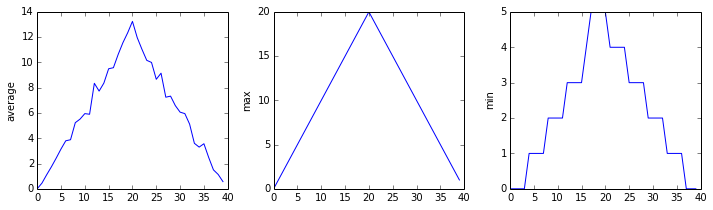
\includegraphics[scale=0.5]{novice/python/img/inflammation-loop-01.png}
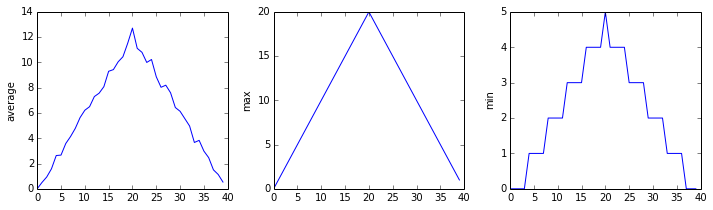
\includegraphics[scale=0.5]{novice/python/img/inflammation-loop-02.png}
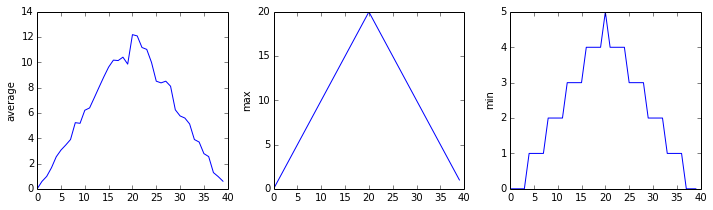
\includegraphics[scale=0.5]{novice/python/img/inflammation-loop-03.png}
\caption{Inflammation Statistics for First Three Data Sets}\label{f:inflammation-loop}
\end{center}
\end{figure}

Sure enough, the maxima of these data sets show exactly the same ramp as
the first, and their minima show the same staircase structure.

\begin{challenge}
  Write a function called \texttt{analyze\_all} that takes a filename
  pattern as its sole argument and runs \texttt{analyze} for each file
  whose name matches the pattern.
\end{challenge}

\begin{keypoints}
\begin{swcitemize}
\item
  Use \texttt{for variable in collection} to process the elements of a
  collection one at a time.
\item
  The body of a for loop must be indented.
\item
  Use \texttt{len(thing)} to determine the length of something that
  contains other values.
\item
  \texttt{{[}value1, value2, value3, ...{]}} creates a list.
\item
  Lists are indexed and sliced in the same way as strings and arrays.
\item
  Lists are mutable (i.e., their values can be changed in place).
\item
  Strings are immutable (i.e., the characters in them cannot be
  changed).
\item
  Use \texttt{glob.glob(pattern)} to create a list of files whose names
  match a pattern.
\item
  Use \texttt{*} in a pattern to match zero or more characters, and
  \texttt{?} to match any single character.
\end{swcitemize}
\end{keypoints}

\section{Making Choices}

Our previous lessons have shown us how to manipulate data, define our
own functions, and repeat things. However, the programs we have written
so far always do the same things, regardless of what data they're given.
We want programs to make choices based on the values they are
manipulating. To help us see what decisions they're making, we'll start
by looking at how computers manipulate images.

\begin{objectives}
\begin{swcitemize}
\item
  Create a simple ``image'' made out of colored blocks.
\item
  Explain how the RGB model represents colors.
\item
  Explain the similarities and differences between tuples and lists.
\item
  Write conditional statements including \texttt{if}, \texttt{elif}, and
  \texttt{else} branches.
\item
  Correctly evaluate expressions containing \texttt{and} and
  \texttt{or}.
\item
  Correctly write and interpret code containing nested loops and
  conditionals.
\item
  Explain the advantages of putting frequently-modified code in a
  function.
\end{swcitemize}
\end{objectives}

\subsection{Image Grids}

Let's start by creating some simple heat maps of our own using a library
called \texttt{ipythonblocks}. The first step is to create our own
``image'':

\begin{VerbIn}
from ipythonblocks import ImageGrid
\end{VerbIn}

Unlike the \texttt{import} statements we have seen earlier, this one
doesn't load the entire \texttt{ipythonblocks} library. Instead, it just
loads \texttt{ImageGrid} from that library, since that's the only thing
we need (for now).

Once we have \texttt{ImageGrid} loaded, we can use it to create a very
simple grid of colored cells:

\begin{VerbIn}
grid = ImageGrid(5, 3)
grid.show()
\end{VerbIn}

% FIXME
\begin{Verbatim}
table.blockgrid {border: none;} .blockgrid tr {border: none;} .blockgrid td {padding: 0px;} #blocks84e827e4-60f2-4e82-b41a-c95955a972aa td {border: 1px solid white;}
\end{Verbatim}

Just like a NumPy array, an \texttt{ImageGrid} has some properties that
hold information about it:

\begin{VerbIn}
print 'grid width:', grid.width
print 'grid height:', grid.height
print 'grid lines on:', grid.lines_on
\end{VerbIn}

\begin{VerbOut}
grid width: 5
grid height: 3
grid lines on: True
\end{VerbOut}

The obvious thing to do with a grid like this is color in its cells,
but in order to do that, we need to know how computers represent
color. The most common schemes are \gl{RGB}{g:rgb}, which is short for
``red, green, blue''. RGB is an \gl{additive color model}{g:additive-color-model}:
every shade is some combination of red, green, and blue
intensities. We can think of these three values as being the axes in a
cube (\figref{f:color-cube}).

\swcgraphics{f:color-cube}{The RGB Color Cube}{novice/python/img/color-cube.png}{1.0}

An RGB color is an example of a multi-part value: like a Cartesian
coordinate, it is one thing with several parts. We can represent such a
value in Python using a \gl{tuple}{g:tuple}, which we write using
parentheses instead of the square brackets used for a list:

\begin{VerbIn}
position = (12.3, 45.6)
print 'position is:', position
color = (10, 20, 30)
print 'color is:', color
\end{VerbIn}

\begin{VerbOut}
position is: (12.3, 45.6)
color is: (10, 20, 30)
\end{VerbOut}

We can select elements from tuples using indexing, just as we do with
lists and arrays:

\begin{VerbIn}
print 'first element of color is:', color[0]
\end{VerbIn}

\begin{VerbOut}
first element of color is: 10
\end{VerbOut}

Unlike lists and arrays, though, tuples cannot be changed after they are
created---in technical terms, they are
\gl{immutable}{g:immutable}:

\begin{VerbIn}
color[0] = 40
print 'first element of color after change:', color[0]
\end{VerbIn}

\begin{VerbErr}
---------------------------------------------------------------------------
TypeError                                 Traceback (most recent call last)
<ipython-input-11-9c3dd30a4e52> in <module>()
----> 1 color[0] = 40
      2 print 'first element of color after change:', color[0]

TypeError: 'tuple' object does not support item assignment
\end{VerbErr}

If a tuple represents an RGB color, its red, green, and blue components
can take on values between 0 and 255. The upper bound may seem odd, but
it's the largest number that can be represented in an 8-bit byte (i.e.,
2\textsuperscript{8}-1). This makes it easy for computers to manipulate
colors, while providing fine enough gradations to fool most human eyes,
most of the time.

Let's see what a few RGB colors actually look like:

\begin{VerbIn}
row = ImageGrid(8, 1)
row[0, 0] = (0, 0, 0)   # no color => black
row[1, 0] = (255, 255, 255) # all colors => white
row[2, 0] = (255, 0, 0) # all red
row[3, 0] = (0, 255, 0) # all green
row[4, 0] = (0, 0, 255) # all blue
row[5, 0] = (255, 255, 0) # red and green
row[6, 0] = (255, 0, 255) # red and blue
row[7, 0] = (0, 255, 255) # green and blue
row.show()
\end{VerbIn}

% FIXME
\begin{Verbatim}
table.blockgrid {border: none;} .blockgrid tr {border: none;} .blockgrid td {padding: 0px;} #blocks9d1f4bb1-553c-4074-aec0-dc48fde66e06 td {border: 1px solid white;}
\end{Verbatim}

Simple color values like \texttt{(0,255,0)} are easy enough to decipher
with a bit of practice, but what color is \texttt{(214,90,127)}? To help
us, \texttt{ipythonblocks} provides a function called
\texttt{show\_color}:

\begin{VerbIn}
from ipythonblocks import show_color
show_color(214, 90, 127)
\end{VerbIn}

% FIXME: image

It also provides a table of standard colors:

\begin{VerbIn}
from ipythonblocks import colors
c = ImageGrid(3, 2)
c[0, 0] = colors['Fuchsia']
c[0, 1] = colors['Salmon']
c[1, 0] = colors['Orchid']
c[1, 1] = colors['Lavender']
c[2, 0] = colors['LimeGreen']
c[2, 1] = colors['HotPink']
c.show()
\end{VerbIn}

% FIXME
\begin{Verbatim}
table.blockgrid {border: none;} .blockgrid tr {border: none;} .blockgrid td {padding: 0px;} #blocksb8c954b3-f908-4ab1-8013-65bf49ec1b2f td {border: 1px solid white;}
\end{Verbatim}

\begin{challenge}
  Fill in the \texttt{\_\_\_\_} in the code below to create a bar that
  changes color from dark blue to black.

\begin{VerbIn}
bar = ImageGrid(10, 1)
for x in range(10):
    bar[x, 0] = (0, 0, ____)
bar.show()
\end{VerbIn}
\end{challenge}

\begin{challenge}
  Why do computers use red, green, and blue as their primary colors?
\end{challenge}

\subsection{Conditionals}

The other thing we need in order to create a heat map of our own is a
way to pick a color based on a data value. The tool Python gives us for
doing this is called a \gl{conditional
statement}{g:conditional-statement}, and looks like this:

\begin{VerbIn}
num = 37
if num > 100:
    print 'greater'
else:
    print 'not greater'
print 'done'
\end{VerbIn}

\begin{VerbOut}
not greater
done
\end{VerbOut}

The second line of this code uses the keyword \texttt{if} to tell Python
that we want to make a choice. If the test that follows it is true, the
body of the \texttt{if} (i.e., the lines indented underneath it) are
executed. If the test is false, the body of the \texttt{else} is
executed instead, so only one or the other is ever executed (\figref{f:conditional}).

\swcgraphics{f:conditional}{Flow of Control in a Conditional}{novice/python/img/python-flowchart-conditional.pdf}{0.75}

Conditional statements don't have to include an \texttt{else}. If there
isn't one, Python simply does nothing if the test is false:

\begin{VerbIn}
num = 53
print 'before conditional...'
if num > 100:
    print '53 is greater than 100'
print '...after conditional'
\end{VerbIn}

\begin{VerbOut}
before conditional...
...after conditional
\end{VerbOut}

We can also chain several tests together using \texttt{elif}, which is
short for ``else if''. This makes it simple to write a function that
returns the sign of a number:

\begin{VerbIn}
def sign(num):
    if num > 0:
        return 1
    elif num == 0:
        return 0
    else:
        return -1

print 'sign of -3:', sign(-3)
\end{VerbIn}

\begin{VerbOut}
sign of -3: -1
\end{VerbOut}

One important thing to notice the code above is that we use a double
equals sign \texttt{==} to test for equality rather than a single equals
sign because the latter is used to mean assignment. This convention was
inherited from C, and while many other programming languages work the
same way, it does take a bit of getting used to\ldots{}

We can also combine tests using \texttt{and} and \texttt{or}.
\texttt{and} is only true if both parts are true:

\begin{VerbIn}
if (1 > 0) and (-1 > 0):
    print 'both parts are true'
else:
    print 'one part is not true'
\end{VerbIn}

\begin{VerbOut}
one part is not true
\end{VerbOut}

while \texttt{or} is true if either part is true:

\begin{VerbIn}
if (1 < 0) or ('left' < 'right'):
    print 'at least one test is true'
\end{VerbIn}

\begin{VerbOut}
at least one test is true
\end{VerbOut}

In this case, ``either'' means ``either or both'', not ``either one or
the other but not both''.

\begin{challenge}
  \texttt{True} and \texttt{False} aren't the only values in Python that
  are true and false. In fact, \emph{any} value can be used in an
  \texttt{if} or \texttt{elif}. After reading and running the code
  below, explain what the rule is for which values are considered true
  and which are considered false. (Note that if the body of a
  conditional is a single statement, we can write it on the same line as
  the \texttt{if}.)

\begin{VerbIn}
if '': print 'empty string is true'
if 'word': print 'word is true'
if []: print 'empty list is true'
if [1, 2, 3]: print 'non-empty list is true'
if 0: print 'zero is true'
if 1: print 'one is true'
\end{VerbIn}
\end{challenge}

\begin{challenge}
  Write a function called \texttt{near} that returns \texttt{True} if
  its first parameter is within 10\% of its second and \texttt{False}
  otherwise. Compare your implementation with your partner's: do you
  return the same answer for all possible pairs of numbers?
\end{challenge}

\subsection{Nesting}

Another thing to realize is that \texttt{if} statements can be combined
with loops just as easily as they can be combined with functions. For
example, if we want to sum the positive numbers in a list, we can write
this:

\begin{VerbIn}
numbers = [-5, 3, 2, -1, 9, 6]
total = 0
for n in numbers:
    if n >= 0:
        total = total + n
print 'sum of positive values:', total
\end{VerbIn}

\begin{VerbOut}
sum of positive values: 20
\end{VerbOut}

We could equally well calculate the positive and negative sums in a
single loop:

\begin{VerbIn}
pos_total = 0
neg_total = 0
for n in numbers:
    if n >= 0:
        pos_total = pos_total + n
    else:
        neg_total = neg_total + n
print 'negative and positive sums are:', neg_total, pos_total
\end{VerbIn}

\begin{VerbOut}
negative and positive sums are: -6 20
\end{VerbOut}

We can even put one loop inside another:

\begin{VerbIn}
for consonant in 'bcd':
    for vowel in 'ae':
        print consonant + vowel
\end{VerbIn}

\begin{VerbOut}
ba
be
ca
ce
da
de
\end{VerbOut}

As \figref{f:nested-loop} shows, the \gl{inner loop}{g:inner-loop} runs
from start to finish each time the \gl{outer loop}{g:outer-loop}
runs once.

\swcgraphics{f:nested-loop}{Execution of Nested Loops}{novice/python/img/python-flowchart-nested-loops.pdf}{0.75}

We can combine nesting and conditionals to create patterns in an image:

\begin{VerbIn}
square = ImageGrid(5, 5)
for x in range(square.width):
    for y in range(square.height):
        if x < y:
            square[x, y] = colors['Fuchsia']
        elif x == y:
            square[x, y] = colors['Olive']
        else:
            square[x, y] = colors['SlateGray']
square.show()
\end{VerbIn}

% FIXME
\begin{Verbatim}
table.blockgrid {border: none;} .blockgrid tr {border: none;} .blockgrid td {padding: 0px;} #blocksa391625e-64d4-47e1-a54a-2953c1aea09c td {border: 1px solid white;}
\end{Verbatim}

This is our first hand-made data visualization: the colors show where
\texttt{x} is less than, equal to, or greater than \texttt{y}.

\begin{challenge}
  Will changing the nesting of the loops in the code above---i.e.,
  wrapping the Y-axis loop around the X-axis loop---change the final
  image? Why or why not?
\end{challenge}

\begin{challenge}
  Python (and most other languages in the C family) provides
  \gl{in-place operators}{g:in-place-operator} that work like
  this:

\begin{VerbIn}
x = 1  # original value
x += 1 # add one to x, assigning result back to x
x *= 3 # multiply x by 3
print x
6
\end{VerbIn}

  Rewrite the code that sums the positive and negative numbers in a list
  using in-place operators. Do you think the result is more or less
  readable than the original?
\end{challenge}

\subsection{Creating a Heat Map}

The last step is to turn our data into something we can see. As in
previous lessons, the first step is to get the data into memory:

\begin{VerbIn}
import numpy as np
data = np.loadtxt(fname='inflammation-01.csv', delimiter=',')
print 'data shape:', data.shape
\end{VerbIn}

\begin{VerbOut}
data shape: (60, 40)
\end{VerbOut}

The second is to create an image grid that is the same size as the data:

\begin{VerbIn}
width, height = data.shape
heatmap = ImageGrid(width, height)
\end{VerbIn}

(The first line of the code above takes advantage of a neat trick: we
can unpack the values in a tuple by assigning it to as many variables as
it has entries.)

The third step is to decide \emph{how} we are going to color the cells
in the heat map. To keep things simple, we will use red, green, and blue
as our colors, and compare data values to the data set's mean. Here's
the code:

\begin{VerbIn}
for x in range(width):
    for y in range(height):
        if data[x, y] < data.mean():
            heatmap[x, y] = colors['Red']
        elif data[x, y] == data.mean():
            heatmap[x, y] = colors['Green']
        else:
            heatmap[x, y] = colors['Blue']
heatmap.show()
\end{VerbIn}

% FIXME
\begin{Verbatim}
table.blockgrid {border: none;} .blockgrid tr {border: none;} .blockgrid td {padding: 0px;} #blocks1cdd8344-bb95-4b16-bc13-b4fb6f13235a td {border: 1px solid white;}
\end{Verbatim}

This may be what we asked for, but both the image and the code are
hideous:

\begin{swcenumerate}
\item
  It's too large for us to view the whole thing at once on a small
  laptop screen.
\item
  Our first heatmap had time along the X axis; this seems to have time
  along the Y axis.
\item
  Red against blue is pretty hard on the eyes.
\item
  The heatmap only shows two colors because none of the (integer)
  measurements has exactly the same value as the (fractional) mean.
\item
  We are calculating the mean of \texttt{data} either once or twice each
  time we go through the loop. That means that on a 40×60 data set, we
  are performing the same calculation 2400 times.
\end{swcenumerate}

Here's how we can improve it:

\begin{swcenumerate}
\item
  We can give \texttt{ImageGrid} an optional parameter
  \texttt{block\_size} to set the size of each block.
\item
  We can transpose our data before creating the grid.
\item
  We can pick better colors (I'm personally fond of orchid, fuchsia, and
  hot pink).
\item
  Instead of checking if values are exactly equal to the mean, we can
  see if they are close to it.
\item
  We can calculate the mean once, before we start our loops, and use
  that value over and over.
\end{swcenumerate}

Our modified code looks like this:

\begin{VerbIn}
flipped = data.transpose()
width, height = flipped.shape
heatmap = ImageGrid(width, height, block_size=5)
center = flipped.mean()
for x in range(width):
    for y in range(height):
        if flipped[x, y] < (0.8 * center):
            heatmap[x, y] = colors['Orchid']
        elif flipped[x, y] > (1.2 * center):
            heatmap[x, y] = colors['HotPink']
        else:
            heatmap[x, y] = colors['Fuchsia']
heatmap.show()
\end{VerbIn}

% FIXME
\begin{Verbatim}
table.blockgrid {border: none;} .blockgrid tr {border: none;} .blockgrid td {padding: 0px;} #blocksa46f17da-750a-4616-8173-7dfb16227fb8 td {border: 1px solid white;}
\end{Verbatim}

That's a bit better---but now the contrast between the colors isn't
great enough. And there still aren't very many fuchsia cells: we may
want to widen the band around the mean that gets that color.

We could rewrite our loop a third time, but the right thing to do is to
put our code in a function so that we can experiment with bands and
colors more easily.

\begin{VerbIn}
def make_heatmap(values, low_color, mid_color, high_color, low_band, high_band, block_size):
    '''Make a 3-colored heatmap from a 2D array of data.'''
    width, height = values.shape
    result = ImageGrid(width, height, block_size=block_size)
    center = values.mean()
    for x in range(width):
        for y in range(height):
            if values[x, y] < low_band * center:
                result[x, y] = low_color
            elif values[x, y] > high_band * center:
                result[x, y] = high_color
            else:
                result[x, y] = mid_color
    return result
\end{VerbIn}

To test this function, we'll run it with the settings we just used:

\begin{VerbIn}
h = make_heatmap(flipped, colors['Orchid'], colors['Fuchsia'], colors['HotPink'], 0.8, 1.2, 5)
h.show()
\end{VerbIn}

% FIXME
\begin{Verbatim}
table.blockgrid {border: none;} .blockgrid tr {border: none;} .blockgrid td {padding: 0px;} #blocks01f46f8f-ce3d-4e60-810e-14913fdd0249 td {border: 1px solid white;}
\end{Verbatim}

That seems right, so let's widen the band and use more dramatic colors:

\begin{VerbIn}
h = make_heatmap(flipped, colors['Gray'], colors['YellowGreen'], colors['SpringGreen'], 0.5, 1.5, 5)
h.show()
\end{VerbIn}

% FIXME
\begin{Verbatim}
table.blockgrid {border: none;} .blockgrid tr {border: none;} .blockgrid td {padding: 0px;} #blocks934bdfbe-fa39-46bc-951f-e504b83c5ed2 td {border: 1px solid white;}
\end{Verbatim}

We'll probably want to experiment a bit more before publishing, but
writing a function has made experimenting easy. We can make it even
easier by re-defining our function one more time to give the parameters
default values. While we're at it, let's put the low and high bands at
the front, since they're more likely to change than our color choices:

\begin{VerbIn}
def make_heatmap(values,
                 low_band=0.5, high_band=1.5,
                 low_color=colors['Gray'], mid_color=colors['YellowGreen'], high_color=colors['SpringGreen'],
                 block_size=5):
    '''Make a 3-colored heatmap from a 2D array of data.
    Default color scheme is gray to green.'''
    width, height = values.shape
    result = ImageGrid(width, height, block_size=block_size)
    center = values.mean()
    for x in range(width):
        for y in range(height):
            if values[x, y] < low_band * center:
                result[x, y] = low_color
            elif values[x, y] > high_band * center:
                result[x, y] = high_color
            else:
                result[x, y] = mid_color
    return result
\end{VerbIn}

Once default values are added, the function's first line is too long to
fit comfortably on our screen. Rather than breaking it wherever it hits
the right edge of the screen, we have divided the parameters into
logical groups to make it more readable.

Again, our first test is to re-run it with the same values as before
(which we give it in a different order, since we've changed the order of
parameters):

\begin{VerbIn}
h = make_heatmap(flipped, 0.5, 1.5, colors['Gray'], colors['YellowGreen'], colors['SpringGreen'], 5)
h.show()
\end{VerbIn}

% FIXME
\begin{Verbatim}
table.blockgrid {border: none;} .blockgrid tr {border: none;} .blockgrid td {padding: 0px;} #blocks68bc8298-2807-40bb-8077-cb6a6c133f91 td {border: 1px solid white;}
\end{Verbatim}

We can now leave out everything except the data being visualized, or
provide the data and the bands and re-use the default colors and block
size:

\begin{VerbIn}
h = make_heatmap(flipped, 0.4, 1.6)
h.show()
\end{VerbIn}

% FIXME
\begin{Verbatim}
table.blockgrid {border: none;} .blockgrid tr {border: none;} .blockgrid td {padding: 0px;} #blocks3a6cb5f4-cba3-448a-b130-320fed0e64e4 td {border: 1px solid white;}
\end{Verbatim}

We can now explore our data with just a few keystrokes, which means we
can concentrate on our science and not on our programming.

\begin{challenge}
  Why did we transpose our data outside our heat map function? Why not
  have the function perform the transpose?
\end{challenge}

\begin{challenge}
  Why does the heat map function return the grid rather than displaying
  it immediately? Do you think this is a good or bad design choice?
\end{challenge}

\begin{challenge}
  Explain what the overall effect of this code is:
\begin{VerbIn}
temp = left
left = right
right = temp
\end{VerbIn}
Compare it to:
\begin{VerbIn}
left, right = right, left
\end{VerbIn}
  Do they always do the same thing?
  Which do you find easier to read?
\end{challenge}

\begin{keypoints}
\begin{swcitemize}
\item
  Use the \texttt{ImageGrid} class from the \texttt{ipythonblocks}
  library to create simple ``images'' made of colored blocks.
\item
  Specify colors use (red, green, blue) triples, each component of which
  is an integer in the range 0..255.
\item
  Use \texttt{if condition} to start a conditional statement,
  \texttt{elif condition} to provide additional tests, and \texttt{else}
  to provide a default.
\item
  The bodies of the branches of conditional statements must be indented.
\item
  Use \texttt{==} to test for equality.
\item
  \texttt{X and Y} is only true if both X and Y are true.
\item
  \texttt{X or Y} is true if either X or Y, or both, are true.
\item
  Zero, the empty string, and the empty list are considered false; all
  other numbers, strings, and lists are considered true.
\item
  Nest loops to operate on multi-dimensional data.
\item
  Put code whose parameters change frequently in a function, then call
  it with different parameter values to customize its behavior.
\end{swcitemize}
\end{keypoints}

\section{Defensive Programming}

Our previous lessons have introduced the basic tools of programming:
variables and lists, file I/O, loops, conditionals, and functions. What
they \emph{haven't} done is show us how to tell whether a program is
getting the right answer, and how to tell if it's \emph{still} getting
the right answer as we make changes to it.

To achieve that, we need to:

\begin{swcitemize}
\item
  write programs that check their own operation,
\item
  write and run tests for widely-used functions, and
\item
  make sure we know what ``correct'' actually means.
\end{swcitemize}

The good news is, doing these things will speed up our programming, not
slow it down. As in real carpentry---the kind done with lumber---the
time saved by measuring carefully before cutting a piece of wood is much
greater than the time that measuring takes.

\begin{objectives}
\begin{swcitemize}
\item
  Explain what an assertion is.
\item
  Add assertions to programs that correctly check the program's state.
\item
  Correctly add precondition and postcondition assertions to functions.
\item
  Explain what test-driven development is, and use it when creating new
  functions.
\item
  Explain why variables should be initialized using actual data values
  rather than arbitrary constants.
\item
  Debug code containing an error systematically.
\end{swcitemize}
\end{objectives}

\subsection{Assertions}

The first step toward getting the right answers from our programs is to
assume that mistakes \emph{will} happen and to guard against them. This
is called \gl{defensive programming}{g:defensive-programming}, and
the most common way to do it is to add
\gl{assertions}{g:assertion} to our code so that it checks itself
as it runs. An assertion is simply a statement that something must be
true at a certain point in a program. When Python sees one, it checks
that the assertion's condition. If it's true, Python does nothing, but
if it's false, Python halts the program immediately and prints the error
message provided. For example, this piece of code halts as soon as the
loop encounters a value that isn't positive:

\begin{VerbIn}
numbers = [1.5, 2.3, 0.7, -0.001, 4.4]
total = 0.0
for n in numbers:
    assert n >= 0.0, 'Data should only contain positive values'
    total += n
print 'total is:', total
\end{VerbIn}

\begin{VerbErr}
---------------------------------------------------------------------------
AssertionError                            Traceback (most recent call last)
<ipython-input-3-33d87ea29ae4> in <module>()
      2 total = 0.0
      3 for n in numbers:
----> 4     assert n >= 0.0, 'Data should only contain positive values'
      5     total += n
      6 print 'total is:', total

AssertionError: Data should only contain positive values
\end{VerbErr}

Programs like the Firefox browser are full of assertions: 10-20\% of the
code they contain are there to check that the other 80-90\% are working
correctly. Broadly speaking, assertions fall into three categories:

\begin{swcitemize}
\item
  A \gl{precondition}{g:precondition} is something that must be
  true at the start of a function in order for it to work correctly.
\item
  A \gl{postcondition}{g:postcondition} is something that the
  function guarantees is true when it finishes.
\item
  An \gl{invariant}{g:invariant} is something that is always true
  at a particular point inside a piece of code.
\end{swcitemize}

For example, suppose we are representing rectangles using a tuple of
four coordinates \texttt{(x0, y0, x1, y1)}. In order to do some
calculations, we need to normalize the rectangle so that it is at the
origin and 1.0 units long on its longest axis. This function does that,
but checks that its input is correctly formatted and that its result
makes sense:

\begin{VerbIn}
def normalize_rectangle(rect):
    '''Normalizes a rectangle so that it is at the origin and 1.0 units long on its longest axis.'''
    assert len(rect) == 4, 'Rectangles must contain 4 coordinates'
    x0, y0, x1, y1 = rect
    assert x0 < x1, 'Invalid X coordinates'
    assert y0 < y1, 'Invalid Y coordinates'

    dx = x1 - x0
    dy = y1 - y0
    if dx > dy:
        scaled = float(dx) / dy
        upper_x, upper_y = 1.0, scaled
    else:
        scaled = float(dx) / dy
        upper_x, upper_y = scaled, 1.0

    assert 0 < upper_x <= 1.0, 'Calculated upper X coordinate invalid'
    assert 0 < upper_y <= 1.0, 'Calculated upper Y coordinate invalid'

    return (0, 0, upper_x, upper_y)
\end{VerbIn}

The preconditions on lines 2, 4, and 5 catch invalid inputs:

\begin{VerbIn}
print normalize_rectangle( (0.0, 1.0, 2.0) ) # missing the fourth coordinate
\end{VerbIn}

\begin{VerbErr}
---------------------------------------------------------------------------
AssertionError                            Traceback (most recent call last)
<ipython-input-5-3a97b1dcab70> in <module>()
----> 1 print normalize_rectangle( (0.0, 1.0, 2.0) ) # missing the fourth coordinate

<ipython-input-4-9f8adbfdcfc9> in normalize_rectangle(rect)
      1 def normalize_rectangle(rect):
      2     '''Normalizes a rectangle so that it is at the origin and 1.0 units long on its longest axis.'''
----> 3     assert len(rect) == 4, 'Rectangles must contain 4 coordinates'
      4     x0, y0, x1, y1 = rect
      5     assert x0 < x1, 'Invalid X coordinates'

AssertionError: Rectangles must contain 4 coordinates
\end{VerbErr}

\begin{VerbIn}
print normalize_rectangle( (4.0, 2.0, 1.0, 5.0) ) # X axis inverted
\end{VerbIn}

\begin{VerbErr}
---------------------------------------------------------------------------
AssertionError                            Traceback (most recent call last)
<ipython-input-6-f05ae7878a45> in <module>()
----> 1 print normalize_rectangle( (4.0, 2.0, 1.0, 5.0) ) # X axis inverted

<ipython-input-4-9f8adbfdcfc9> in normalize_rectangle(rect)
      3     assert len(rect) == 4, 'Rectangles must contain 4 coordinates'
      4     x0, y0, x1, y1 = rect
----> 5     assert x0 < x1, 'Invalid X coordinates'
      6     assert y0 < y1, 'Invalid Y coordinates'
      7

AssertionError: Invalid X coordinates
\end{VerbErr}

The post-conditions help us catch bugs by telling us when our
calculations cannot have been correct. For example, if we normalize a
rectangle that is taller than it is wide everything seems OK:

\begin{VerbIn}
print normalize_rectangle( (0.0, 0.0, 1.0, 5.0) )
\end{VerbIn}

\begin{VerbOut}
(0, 0, 0.2, 1.0)
\end{VerbOut}

but if we normalize one that's wider than it is tall, the assertion is
triggered:

\begin{VerbIn}
print normalize_rectangle( (0.0, 0.0, 5.0, 1.0) )
\end{VerbIn}

\begin{VerbErr}
---------------------------------------------------------------------------
AssertionError                            Traceback (most recent call last)
<ipython-input-8-5f0ef7954aeb> in <module>()
----> 1 print normalize_rectangle( (0.0, 0.0, 5.0, 1.0) )

<ipython-input-4-9f8adbfdcfc9> in normalize_rectangle(rect)
     16
     17     assert 0 < upper_x <= 1.0, 'Calculated upper X coordinate invalid'
---> 18     assert 0 < upper_y <= 1.0, 'Calculated upper Y coordinate invalid'
     19
     20     return (0, 0, upper_x, upper_y)

AssertionError: Calculated upper Y coordinate invalid
\end{VerbErr}

Re-reading our function, we realize that line 10 should divide
\texttt{dy} by \texttt{dx} rather than \texttt{dx} by \texttt{dy}. (You
can display line numbers by typing Ctrl-M, then L.) If we had left out
the assertion at the end of the function, we would have created and
returned something that had the right shape as a valid answer, but
wasn't. Detecting and debugging that would almost certainly have taken
more time in the long run than writing the assertion.

But assertions aren't just about catching errors: they also help people
understand programs. Each assertion gives the person reading the program
a chance to check (consciously or otherwise) that their understanding
matches what the code is doing.

Most good programmers follow two rules when adding assertions to their
code. The first is, ``\urlfoot{../../rules.html\#fail-early-fail-often}{fail
early, fail often}''. The greater the distance between when and where an
error occurs and when it's noticed, the harder the error will be to
debug, so good code catches mistakes as early as possible.

The second rule is,
``\urlfoot{../../rules.html\#turn-bugs-into-assertions-or-tests}{turn bugs
into assertions or tests}''. If you made a mistake in a piece of code,
the odds are good that you have made other mistakes nearby, or will make
the same mistake (or a related one) the next time you change it. Writing
assertions to check that you haven't \gl{regressed}{g:regression}
(i.e., haven't re-introduced an old problem) can save a lot of time in
the long run, and helps to warn people who are reading the code
(including your future self) that this bit is tricky.

\begin{challenge}
  Suppose you are writing a function called \texttt{average} that
  calculates the average of the numbers in a list. What pre-conditions
  and post-conditions would you write for it? Compare your answer to
  your neighbor's: can you think of a function that will past your tests
  but not hers or vice versa?
\end{challenge}

\begin{challenge}
  Explain in words what the assertions in this code check, and for each
  one, give an example of input that will make that assertion fail.

\begin{VerbIn}
def running(values):
    assert len(values) > 0
    result = [values[0]]
    for v in values[1:]:
        assert result[-1] >= 0
        result.append(result[-1] + v)
    assert result[-1] >= result[0]
    return result
\end{VerbIn}
\end{challenge}

\subsection{Test-Driven Development}

An assertion checks that something is true at a particular point in the
program. The next step is to check the overall behavior of a piece of
code, i.e., to make sure that it produces the right output when it's
given a particular input. For example, suppose we need to find where two
or more time series overlap. The range of each time series is
represented as a pair of numbers, which are the time the interval
started and ended. The output is the largest range that they all
include (\figref{f:overlapping-ranges}).

\swcgraphics{f:overlapping-ranges}{Overlapping Ranges}{novice/python/img/python-overlapping-ranges.pdf}{0.75}

Most novice programmers would solve this problem like this:

\begin{swcenumerate}
\item
  Write a function \texttt{range\_overlap}.
\item
  Call it interactively on two or three different inputs.
\item
  If it produces the wrong answer, fix the function and re-run that
  test.
\end{swcenumerate}

This clearly works---after all, thousands of scientists are doing it
right now---but there's a better way:

\begin{swcenumerate}
\item
  Write a short function for each test.
\item
  Write a \texttt{range\_overlap} function that should pass those tests.
\item
  If \texttt{range\_overlap} produces any wrong answers, fix it and
  re-run the test functions.
\end{swcenumerate}

Writing the tests \emph{before} writing the function they exercise is
called \gl{test-driven development}{g:test-driven-development}
(TDD). Its advocates believe it produces better code faster because:

\begin{swcenumerate}
\item
  If people write tests after writing the thing to be tested, they are
  subject to confirmation bias, i.e., they subconsciously write tests to
  show that their code is correct, rather than to find errors.
\item
  Writing tests helps programmers figure out what the function is
  actually supposed to do.
\end{swcenumerate}

Here are three test functions for \texttt{range\_overlap}:

\begin{VerbIn}
assert range_overlap([ (0.0, 1.0) ]) == (0.0, 1.0)
assert range_overlap([ (0.0, 1.0), (0.0, 2.0) ]) == (0.0, 1.0)
assert range_overlap([ (0.0, 1.0), (0.0, 2.0), (-1.0, 1.0) ]) == (0.0, 1.0)
\end{VerbIn}

The error is actually reassuring: we haven't written
\texttt{range\_overlap} yet, so if the tests passed, it would be a sign
that someone else had and that we were accidentally using their
function.

And as a bonus of writing these tests, we've implicitly defined what our
input and output look like: we expect a list of pairs as input, and
produce a single pair as output.

Something important is missing, though. We don't have any tests for the
case where the ranges don't overlap at all:

\begin{VerbIn}
assert range_overlap([ (0.0, 1.0), (5.0, 6.0) ]) == ???
\end{VerbIn}

What should \texttt{range\_overlap} do in this case: fail with an error
message, produce a special value like \texttt{(0.0, 0.0)} to signal that
there's no overlap, or something else? Any actual implementation of the
function will do one of these things; writing the tests first helps us
figure out which is best \emph{before} we're emotionally invested in
whatever we happened to write before we realized there was an issue.

And what about this case?

\begin{VerbIn}
assert range_overlap([ (0.0, 1.0), (1.0, 2.0) ]) == ???
\end{VerbIn}

Do two segments that touch at their endpoints overlap or not?
Mathematicians usually say ``yes'', but engineers usually say ``no''.
The best answer is ``whatever is most useful in the rest of our
program'', but again, any actual implementation of
\texttt{range\_overlap} is going to do \emph{something}, and whatever it
is ought to be consistent with what it does when there's no overlap at
all.

Since we're planning to use the range this function returns as the X
axis in a time series chart, we decide that:

\begin{swcenumerate}
\item
  every overlap has to have non-zero width, and
\item
  we will return the special value \texttt{None} when there's no
  overlap.
\end{swcenumerate}

\texttt{None} is built into Python, and means ``nothing here''. (Other
languages often call the equivalent value \texttt{null} or
\texttt{nil}). With that decision made, we can finish writing our last
two tests:

\begin{VerbIn}
assert range_overlap([ (0.0, 1.0), (5.0, 6.0) ]) == None
assert range_overlap([ (0.0, 1.0), (1.0, 2.0) ]) == None
\end{VerbIn}

\begin{VerbErr}
---------------------------------------------------------------------------
AssertionError                            Traceback (most recent call last)
<ipython-input-10-d877ef460ba2> in <module>()
----> 1 assert range_overlap([ (0.0, 1.0), (5.0, 6.0) ]) == None
      2 assert range_overlap([ (0.0, 1.0), (1.0, 2.0) ]) == None

AssertionError: 
\end{VerbErr}

Again, we get an error because we haven't written our function, but
we're now ready to do so:

\begin{VerbIn}
def range_overlap(ranges):
    '''Return common overlap among a set of [low, high] ranges.'''
    lowest = 0.0
    highest = 1.0
    for (low, high) in ranges:
        lowest = max(lowest, low)
        highest = min(highest, high)
    return (lowest, highest)
\end{VerbIn}

(Take a moment to think about why we use \texttt{max} to raise
\texttt{lowest} and \texttt{min} to lower \texttt{highest}.) We'd now
like to re-run our tests, but they're scattered across three different
cells. To make running them easier, let's put them all in a function:

\begin{VerbIn}
def test_range_overlap():
    assert range_overlap([ (0.0, 1.0) ]) == (0.0, 1.0)
    assert range_overlap([ (0.0, 1.0), (0.0, 2.0) ]) == (0.0, 1.0)
    assert range_overlap([ (0.0, 1.0), (0.0, 2.0), (-1.0, 1.0) ]) == (0.0, 1.0)
    assert range_overlap([ (0.0, 1.0), (5.0, 6.0) ]) == None
    assert range_overlap([ (0.0, 1.0), (1.0, 2.0) ]) == None
\end{VerbIn}

We can now test \texttt{range\_overlap} with a single function call:

\begin{VerbIn}
test_range_overlap()
\end{VerbIn}

\begin{VerbErr}
---------------------------------------------------------------------------
AssertionError                            Traceback (most recent call last)
<ipython-input-13-cf9215c96457> in <module>()
----> 1 test_range_overlap()

<ipython-input-12-34c3659163fc> in test_range_overlap()
      3     assert range_overlap([ (0.0, 1.0), (0.0, 2.0) ]) == (0.0, 1.0)
      4     assert range_overlap([ (0.0, 1.0), (0.0, 2.0), (-1.0, 1.0) ]) == (0.0, 1.0)
----> 5     assert range_overlap([ (0.0, 1.0), (5.0, 6.0) ]) == None
      6     assert range_overlap([ (0.0, 1.0), (1.0, 2.0) ]) == None

AssertionError: 
\end{VerbErr}

The first of the tests that was supposed to produce \texttt{None} fails,
so we know there's something wrong with our function. What we
\emph{don't} know, though, is whether the last of our five tests passed
or failed, because Python halted the program as soon as it spotted the
first error. Still, some information is better than none, and if we
trace the behavior of the function with that input, we realize that
we're initializing \texttt{lowest} and \texttt{highest} to 0.0 and 1.0
respectively, regardless of the input values. This violates another
important rule of programming:
``\urlfoot{../../rules.html\#always-initialize-from-data}{always initialize
from data}''. We'll leave it as an exercise to fix
\texttt{range\_overlap}.

\begin{challenge}
  Fix \texttt{range\_overlap}. Re-run \texttt{test\_range\_overlap}
  after each change you make.
\end{challenge}

\subsection{Debugging}

Once testing has uncovered problems, the next step is to fix them. Many
novices do this by making more-or-less random changes to their code
until it seems to produce the right answer, but that's very inefficient
(and the result is usually only correct for the one case they're
testing). The more experienced a programmer is, the more systematically
they debug, and most follow some variation on the rules explained below.

\subsection*{Know What It's Supposed to Do}

The first step in debugging something is to
\urlfoot{../../rules.html\#know-what-its-supposed-to-do}{know what it's
supposed to do}. ``My program doesn't work'' isn't good enough: in order
to diagnose and fix problems, we need to be able to tell correct output
from incorrect. If we can write a test case for the failing case---i.e.,
if we can assert that with \emph{these} inputs, the function should
produce \emph{that} result--- then we're ready to start debugging. If we
can't, then we need to figure out how we're going to know when we've
fixed things.

But writing test cases for scientific software is frequently harder than
writing test cases for commercial applications, because if we knew what
the output of the scientific code was supposed to be, we wouldn't be
running the software: we'd be writing up our results and moving on to
the next program. In practice, scientists tend to do the following:

\begin{swcenumerate}
\item
  \emph{Test with simplified data.} Before doing statistics on a real
  data set, we should try calculating statistics for a single record,
  for two identical records, for two records whose values are one step
  apart, or for some other case where we can calculate the right answer
  by hand.
\item
  \emph{Test a simplified case.} If our program is supposed to simulate
  magnetic eddies in rapidly-rotating blobs of supercooled helium, our
  first test should be a blob of helium that isn't rotating, and isn't
  being subjected to any external electromagnetic fields. Similarly, if
  we're looking at the effects of climate change on speciation, our
  first test should hold temperature, precipitation, and other factors
  constant.
\item
  \emph{Compare to an oracle.} A \gl{test oracle}{g:test-oracle}
  is something---experimental data, an older program whose results are
  trusted, or even a human expert---against which we can compare the
  results of our new program. If we have a test oracle, we should store
  its output for particular cases so that we can compare it with our new
  results as often as we like without re-running that program.
\item
  \emph{Check conservation laws.} Mass, energy, and other quantitites
  are conserved in physical systems, so they should be in programs as
  well. Similarly, if we are analyzing patient data, the number of
  records should either stay the same or decrease as we move from one
  analysis to the next (since we might throw away outliers or records
  with missing values). If ``new'' patients start appearing out of
  nowhere as we move through our pipeline, it's probably a sign that
  something is wrong.
\item
  \emph{Visualize.} Data analysts frequently use simple visualizations
  to check both the science they're doing and the correctness of their
  code (just as we did in the \urlfoot{01-numpy.html}{opening lesson} of
  this tutorial). This should only be used for debugging as a last
  resort, though, since it's very hard to compare two visualizations
  automatically.
\end{swcenumerate}

\subsection*{Make It Fail Every Time}

We can only debug something when it fails, so the second step is always
to find a test case that
\urlfoot{../../rules.html\#make-it-fail-every-time}{makes it fail every
time}. The ``every time'' part is important because few things are more
frustrating than debugging an intermittent problem: if we have to call a
function a dozen times to get a single failure, the odds are good that
we'll scroll past the failure when it actually occurs.

As part of this, it's always important to check that our code is
``plugged in'', i.e., that we're actually exercising the problem that we
think we are. Every programmer has spent hours chasing a bug, only to
realize that they were actually calling their code on the wrong data set
or with the wrong configuration parameters, or are using the wrong
version of the software entirely. Mistakes like these are particularly
likely to happen when we're tired, frustrated, and up against a
deadline, which is one of the reasons late-night (or overnight) coding
sessions are almost never worthwhile.

\subsection*{Make It Fail Fast}

If it takes 20 minutes for the bug to surface, we can only do three
experiments an hour. That doesn't must mean we'll get less data in more
time: we're also more likely to be distracted by other things as we wait
for our program to fail, which means the time we \emph{are} spending on
the problem is less focused. It's therefore critical to
\urlfoot{../../rules.html\#make-it-fail-fast}{make it fail fast}.

As well as making the program fail fast in time, we want to make it fail
fast in space, i.e., we want to localize the failure to the smallest
possible region of code:

\begin{swcenumerate}
\item
  The smaller the gap between cause and effect, the easier the
  connection is to find. Many programmers therefore use a divide and
  conquer strategy to find bugs, i.e., if the output of a function is
  wrong, they check whether things are OK in the middle, then
  concentrate on either the first or second half, and so on.
\item
  N things can interact in N\textsuperscript{2/2} different ways, so
  every line of code that \emph{isn't} run as part of a test means more
  than one thing we don't need to worry about.
\end{swcenumerate}

\subsection*{Change One Thing at a Time, For a Reason}

Replacing random chunks of code is unlikely to do much good. (After all,
if you got it wrong the first time, you'll probably get it wrong the
second and third as well.) Good programmers therefore
\urlfoot{../../rules.html\#change-one-thing-at-a-time}{change one thing at
a time, for a reason} They are either trying to gather more information
(``is the bug still there if we change the order of the loops?'') or
test a fix (``can we make the bug go away by sorting our data before
processing it?'').

Every time we make a change, however small, we should re-run our tests
immediately, because the more things we change at once, the harder it is
to know what's responsible for what (those N\textsuperscript{2}
interactions again). And we should re-run \emph{all} of our tests: more
than half of fixes made to code introduce (or re-introduce) bugs, so
re-running all of our tests tells us whether we have
\gl{regressed}{g:regression}.

\subsection*{Keep Track of What You've Done}

Good scientists keep track of what they've done so that they can
reproduce their work, and so that they don't waste time repeating the
same experiments or running ones whose results won't be interesting.
Similarly, debugging works best when we
\urlfoot{../../rules.html\#keep-track-of-what-youve-done}{keep track of
what we've done} and how well it worked. If we find ourselves asking,
``Did left followed by right with an odd number of lines cause the
crash? Or was it right followed by left? Or was I using an even number
of lines?'' then it's time to step away from the computer, take a deep
breath, and start working more systematically.

Records are particularly useful when the time comes to ask for help.
People are more likely to listen to us when we can explain clearly what
we did, and we're better able to give them the information they need to
be useful.

\begin{swcbox}{Version Control Revisited}

Version control is often used to reset software to a known state during
debugging, and to explore recent changes to code that might be
responsible for bugs. In particular, most version control systems have a
\texttt{blame} command that will show who last changed particular lines
of code\ldots{}

\end{swcbox}

\subsection*{Be Humble}

And speaking of help: if we can't find a bug in 10 minutes, we should
\urlfoot{../../rules.html\#be-humble}{be humble} and ask for help. Just
explaining the problem aloud is often useful, since hearing what we're
thinking helps us spot inconsistencies and hidden assumptions.

Asking for help also helps alleviate confirmation bias. If we have just
spent an hour writing a complicated program, we want it to work, so
we're likely to keep telling ourselves why it should, rather than
searching for the reason it doesn't. People who aren't emotionally
invested in the code can be more objective, which is why they're often
able to spot the simple mistakes we have overlooked.

Part of being humble is learning from our mistakes. Programmers tend to
get the same things wrong over and over: either they don't understand
the language and libraries they're working with, or their model of how
things work is wrong. In either case, taking note of why the error
occurred and checking for it next time quickly turns into not making the
mistake at all.

And that is what makes us most productive in the long run. As the saying
goes, ``\urlfoot{../../rules.html\#week-hard-work-hour-thought}{A week of
hard work can sometimes save you an hour of thought}.'' If we train
ourselves to avoid making some kinds of mistakes, to break our code into
modular, testable chunks, and to turn every assumption (or mistake) into
an assertion, it will actually take us \emph{less} time to produce
working programs, not more.

\begin{keypoints}
\begin{swcitemize}
\item
  Program defensively, i.e., assume that errors are going to arise, and
  write code to detect them when they do.
\item
  Put assertions in programs to check their state as they run, and to
  help readers understand how those programs are supposed to work.
\item
  Use preconditions to check that the inputs to a function are safe to
  use.
\item
  Use postconditions to check that the output from a function is safe to
  use.
\item
  Write tests before writing code in order to help determine exactly
  what that code is supposed to do.
\item
  Know what code is supposed to do \emph{before} trying to debug it.
\item
  Make it fail every time.
\item
  Make it fail fast.
\item
  Change one thing at a time, and for a reason.
\item
  Keep track of what you've done.
\item
  Be humble.
\end{swcitemize}
\end{keypoints}

\section{Command-Line Programs}

The IPython Notebook and other interactive tools are great for
prototyping code and exploring data, but sooner or later we will want to
use our program in a pipeline or run it in a shell script to process
thousands of data files. In order to do that, we need to make our
programs work like other Unix command-line tools. For example, we may
want a program that reads a data set and prints the average inflammation
per patient:

\begin{VerbIn}
$ python readings.py --mean inflammation-01.csv
\end{VerbIn}

\begin{VerbOut}
5.45
5.425
6.1
...
6.4
7.05
5.9
\end{VerbOut}

but we might also want to look at the minimum of the first four lines

\begin{VerbIn}
$ head -4 inflammation-01.csv | python readings.py --min
\end{VerbIn}

or the maximum inflammations in several files one after another:

\begin{VerbIn}
$ python readings.py --max inflammation-*.csv
\end{VerbIn}

Our overall requirements are:

\begin{swcenumerate}
\item
  If no filename is given on the command line, read data from
  \gl{standard input}{g:standard-input}.
\item
  If one or more filenames are given, read data from them and report
  statistics for each file separately.
\item
  Use the \texttt{-{}-min}, \texttt{-{}-mean}, or \texttt{-{}-max} flag
  to determine what statistic to print.
\end{swcenumerate}

To make this work, we need to know how to handle command-line arguments
in a program, and how to get at standard input. We'll tackle these
questions in turn below.

\begin{objectives}
\begin{swcitemize}
\item
  Use the values of command-line arguments in a program.
\item
  Handle flags and files separately in a command-line program.
\item
  Read data from standard input in a program so that it can be used in a
  pipeline.
\end{swcitemize}
\end{objectives}

\subsection{Command-Line Arguments}

Using the text editor of your choice, save the following in a text file:

\begin{VerbIn}
!cat sys-version.py
\end{VerbIn}

\begin{VerbIn}
import sys
print 'version is', sys.version
\end{VerbIn}

The first line imports a library called \texttt{sys}, which is short for
``system''. It defines values such as \texttt{sys.version}, which
describes which version of Python we are running. We can run this script
from within the IPython Notebook like this:

\begin{VerbIn}
%run sys-version.py
\end{VerbIn}

\begin{VerbOut}
version is 2.7.5 |Anaconda 1.8.0 (x86_64)| (default, Oct 24 2013, 07:02:20)
[GCC 4.0.1 (Apple Inc. build 5493)]
\end{VerbOut}

or like this:

\begin{VerbIn}
!ipython sys-version.py
\end{VerbIn}

\begin{VerbOut}
version is 2.7.5 |Anaconda 1.8.0 (x86_64)| (default, Oct 24 2013, 07:02:20)
[GCC 4.0.1 (Apple Inc. build 5493)]
\end{VerbOut}

The first method, \texttt{\%run}, uses a special command in the IPython
Notebook to run a program in a \texttt{.py} file. The second method is
more general: the exclamation mark \texttt{!} tells the Notebook to run
a shell command, and it just so happens that the command we run is
\texttt{ipython} with the name of the script.

Here's another script that does something more interesting:

\begin{VerbIn}
!cat argv-list.py
\end{VerbIn}

\begin{VerbOut}
import sys
print 'sys.argv is', sys.argv
\end{VerbOut}

The strange name \texttt{argv} stands for ``argument values''. Whenever
Python runs a program, it takes all of the values given on the command
line and puts them in the list \texttt{sys.argv} so that the program can
determine what they were. If we run this program with no arguments:

\begin{VerbIn}
!ipython argv-list.py
\end{VerbIn}

\begin{VerbOut}
sys.argv is ['/Users/gwilson/s/bc/python/novice/argv-list.py']
\end{VerbOut}

the only thing in the list is the full path to our script, which is
always \texttt{sys.argv{[}0{]}}. If we run it with a few arguments,
however:

\begin{VerbIn}
!ipython argv-list.py first second third
\end{VerbIn}

\begin{VerbOut}
sys.argv is ['/Users/gwilson/s/bc/python/novice/argv-list.py', 'first', 'second', 'third']
\end{VerbOut}

then Python adds each of those arguments to that magic list.

With this in hand, let's build a version of \texttt{readings.py} that
always prints the per-patient mean of a single data file. The first step
is to write a function that outlines our implementation, and a
placeholder for the function that does the actual work. By convention
this function is usually called \texttt{main}, though we can call it
whatever we want:

\begin{VerbIn}
# readings-01.py
import sys
import numpy as np

def main():
    script = sys.argv[0]
    filename = sys.argv[1]
    data = np.loadtxt(filename, delimiter=',')
    for m in data.mean(axis=1):
        print m
\end{VerbIn}

This function gets the name of the script from \texttt{sys.argv{[}0{]}},
because that's where it's always put, and the name of the file to
process from \texttt{sys.argv{[}1{]}}. Here's a simple test:

\begin{VerbIn}
$ python readings-01.py inflammation-01.csv
\end{VerbIn}

There is no output because we have defined a function, but haven't
actually called it. Let's add a call to \texttt{main}:

\begin{VerbIn}
# readings-02.py
import sys
import numpy as np

def main():
    script = sys.argv[0]
    filename = sys.argv[1]
    data = np.loadtxt(filename, delimiter=',')
    for m in data.mean(axis=1):
        print m

main()
\end{VerbIn}

and run that:

\begin{VerbIn}
$ python readings-02.py inflammation-01.csv
\end{VerbIn}

\begin{VerbOut}
5.45
5.425
6.1
5.9
5.55
6.225
5.975
6.65
6.625
6.525
6.775
5.8
6.225
5.75
5.225
6.3
6.55
5.7
5.85
6.55
5.775
5.825
6.175
6.1
5.8
6.425
6.05
6.025
6.175
6.55
6.175
6.35
6.725
6.125
7.075
5.725
5.925
6.15
6.075
5.75
5.975
5.725
6.3
5.9
6.75
5.925
7.225
6.15
5.95
6.275
5.7
6.1
6.825
5.975
6.725
5.7
6.25
6.4
7.05
5.9
\end{VerbOut}

\begin{swcbox}{The Right Way to Do It}

If our programs can take complex parameters or multiple filenames, we
shouldn't handle \texttt{sys.argv} directly. Instead, we should use
Python's \texttt{argparse} library, which handles common cases in a
systematic way, and also makes it easy for us to provide sensible error
messages for our users.

\end{swcbox}

\begin{challenge}
  Write a command-line program that does addition and subtraction:
\begin{VerbIn}
python arith.py 1 + 2
\end{VerbIn}
\begin{VerbOut}
3
\end{VerbOut}
\begin{VerbIn}
python arith.py 3 - 4
\end{VerbIn}
\begin{VerbOut}
-1
\end{VerbOut}
  What goes wrong if you try to add multiplication using `*' to the
  program?
\end{challenge}

\begin{challenge}
  Using the \texttt{glob} module introduced
  \urlfoot{earlier}{03-loop.ipynb}, write a simple version of \texttt{ls}
  that shows files in the current directory with a particular suffix:
\begin{VerbIn}
$ python my_ls.py py
\end{VerbIn}
\begin{VerbOut}
left.py right.py zero.py
\end{VerbOut}
\end{challenge}

\subsection{Handling Multiple Files}

The next step is to teach our program how to handle multiple files.
Since 60 lines of output per file is a lot to page through, we'll start
by creating three smaller files, each of which has three days of data
for two patients:

\begin{VerbIn}
$ ls small-*.csv
\end{VerbIn}

\begin{VerbOut}
small-01.csv small-02.csv small-03.csv
\end{VerbOut}

\begin{VerbIn}
$ cat small-01.csv
\end{VerbIn}

\begin{VerbOut}
0,0,1
0,1,2
\end{VerbOut}

\begin{VerbIn}
$ python readings-02.py small-01.csv
\end{VerbIn}

\begin{VerbOut}
0.333333333333
1.0
\end{VerbOut}

Using small data files as input also allows us to check our results more
easily: here, for example, we can see that our program is calculating
the mean correctly for each line, whereas we were really taking it on
faith before. This is yet another rule of programming:
``\urlfoot{../../rules.html\#test-simple-first}{test the simple things
first}.''

We want our program to process each file separately, so we need a looop
that executes once for each filename. If we specify the files on the
command line, the filenames will be in \texttt{sys.argv}, but we need to
be careful: \texttt{sys.argv{[}0{]}} will always be the name of our
script, rather than the name of a file. We also need to handle an
unknown number of filenames, since our program could be run for any
number of files.

The solution to both problems is to loop over the contents of
\texttt{sys.argv{[}1:{]}}. The `1' tells Python to start the slice at
location 1, so the program's name isn't included; since we've left off
the upper bound, the slice runs to the end of the list, and includes all
the filenames. Here's our changed program:

\begin{VerbIn}
# readings-03.py
import sys
import numpy as np

def main():
    script = sys.argv[0]
    for filename in sys.argv[1:]:
        data = np.loadtxt(filename, delimiter=',')
        for m in data.mean(axis=1):
            print m

main()
\end{VerbIn}

and here it is in action:

\begin{VerbIn}
$ python readings-03.py small-01.csv small-02.csv
\end{VerbIn}

\begin{VerbOut}
0.333333333333
1.0
13.6666666667
11.0
\end{VerbOut}

Note: at this point, we have created three versions of our script called
\texttt{readings-01.py}, \texttt{readings-02.py}, and
\texttt{readings-03.py}. We wouldn't do this in real life: instead, we
would have one file called \texttt{readings.py} that we committed to
version control every time we got an enhancement working. For teaching,
though, we need all the successive versions side by side.

\begin{challenge}
  Write a program called \texttt{check.py} that takes the names of one
  or more inflammation data files as arguments and checks that all the
  files have the same number of rows and columns. What is the best way
  to test your program?
\end{challenge}

\subsection{Handling Command-Line Flags}

The next step is to teach our program to pay attention to the
\texttt{-{}-min}, \texttt{-{}-mean}, and \texttt{-{}-max} flags. These
always appear before the names of the files, so we could just do this:

\begin{VerbIn}
# readings-04.py
import sys
import numpy as np

def main():
    script = sys.argv[0]
    action = sys.argv[1]
    filenames = sys.argv[2:]

    for f in filenames:
        data = np.loadtxt(f, delimiter=',')

        if action == '--min':
            values = data.min(axis=1)
        elif action == '--mean':
            values = data.mean(axis=1)
        elif action == '--max':
            values = data.max(axis=1)

        for m in values:
            print m

main()
\end{VerbIn}

This works:

\begin{VerbIn}
$ run readings-04.py --max small-01.csv
\end{VerbIn}

\begin{VerbOut}
1.0
2.0
\end{VerbOut}

but there are seveal things wrong with it:

\begin{swcenumerate}
\item
  \texttt{main} is too large to read comfortably.
\item
  If \texttt{action} isn't one of the three recognized flags, the
  program loads each file but does nothing with it (because none of the
  branches in the conditional match). \gl{Silent
  failures}{g:silent-failure} like this are always hard to debug.
\end{swcenumerate}

This version pulls the processing of each file out of the loop into a
function of its own. It also checks that \texttt{action} is one of the
allowed flags before doing any processing, so that the program fails
fast:

\begin{Verbatim}
# readings-05.py
import sys
import numpy as np

def main():
    script = sys.argv[0]
    action = sys.argv[1]
    filenames = sys.argv[2:]
    assert action in ['--min', '--mean', '--max'], \
           'Action is not one of --min, --mean, or --max: ' + action
    for f in filenames:
        process(f, action)

def process(filename, action):
    data = np.loadtxt(filename, delimiter=',')

    if action == '--min':
        values = data.min(axis=1)
    elif action == '--mean':
        values = data.mean(axis=1)
    elif action == '--max':
        values = data.max(axis=1)

    for m in values:
        print m

main()
\end{Verbatim}

This is four lines longer than its predecessor, but broken into more
digestible chunks of 8 and 12 lines.

Python has a module named
\urlfoot{http://docs.python.org/dev/library/argparse.html}{argparse} that
helps handle complex command-line flags. We will not cover this module
in this lesson but you can go to Tshepang Lekhonkhobe's
\urlfoot{http://docs.python.org/dev/howto/argparse.html}{Argparse tutorial}
that is part of Python's Official Documentation.

\begin{challenge}
  Rewrite this program so that it uses \texttt{-n}, \texttt{-m}, and
  \texttt{-x} instead of \texttt{-{}-min}, \texttt{-{}-mean}, and
  \texttt{-{}-max} respectively. Is the code easier to read? Is the
  program easier to understand?
\end{challenge}

\begin{challenge}
  Separately, modify the program so that if no parameters are given
  (i.e., no action is specified and no filenames are given), it prints a
  message explaining how it should be used.
\end{challenge}

\begin{challenge}
  Separately, modify the program so that if no action is given it
  displays the means of the data.
\end{challenge}

\subsection{Handling Standard Input}

The next thing our program has to do is read data from standard input if
no filenames are given so that we can put it in a pipeline, redirect
input to it, and so on. Let's experiment in another script:

\begin{Verbatim}
# count-stdin.py
import sys

count = 0
for line in sys.stdin:
    count += 1

print count, 'lines in standard input'
\end{Verbatim}

This little program reads lines from a special ``file'' called
\texttt{sys.stdin}, which is automatically connected to the program's
standard input. We don't have to open it---Python and the operating
system take care of that when the program starts up--- but we can do
almost anything with it that we could do to a regular file. Let's try
running it from within the IPython notebook as if it were a regular command-line program:

\begin{VerbIn}
!ipython count-stdin.py < small-01.csv
\end{VerbIn}

\begin{VerbOut}
2 lines in standard input
\end{VerbOut}

What if we run it using \texttt{\%run} (again, from within the notebook)?

\begin{VerbIn}
%run count-stdin.py < fractal_1.txt
\end{VerbIn}

\begin{VerbOut}
0 lines in standard input
\end{VerbOut}

As you can see, \texttt{\%run} doesn't understand file redirection:
that's a shell thing.

A common mistake is to try to run something that reads from standard
input like this:

\begin{VerbIn}
$ python count_stdin.py fractal_1.txt
\end{VerbIn}

i.e., to forget the \texttt{\textless{}} character that redirect the
file to standard input. In this case, there's nothing in standard input,
so the program waits at the start of the loop for someone to type
something on the keyboard. Since there's no way for us to do this, our
program is stuck, and we have to halt it using the \texttt{Interrupt}
option from the \texttt{Kernel} menu in the Notebook.

We now need to rewrite the program so that it loads data from
\texttt{sys.stdin} if no filenames are provided. Luckily,
\texttt{numpy.loadtxt} can handle either a filename or an open file as
its first parameter, so we don't actually need to change
\texttt{process}. That leaves \texttt{main}:

\begin{VerbIn}
# readings-06.py
def main():
    script = sys.argv[0]
    action = sys.argv[1]
    filenames = sys.argv[2:]
    assert action in ['--min', '--mean', '--max'], \
           'Action is not one of --min, --mean, or --max: ' + action
    if len(filenames) == 0:
        process(sys.stdin, action)
    else:
        for f in filenames:
            process(f, action)
\end{VerbIn}

Let's try it out from inside the notebook (we'll see in a moment why we send the output through
\texttt{head}):

\begin{VerbIn}
!ipython readings-06.py --mean < small-01.csv | head -10
\end{VerbIn}

\begin{VerbOut}
[TerminalIPythonApp] CRITICAL | Bad config encountered during initialization:
[TerminalIPythonApp] CRITICAL | Unrecognized flag: '--mean'
=========
 IPython
=========

Tools for Interactive Computing in Python
=========================================

    A Python shell with automatic history (input and output), dynamic object
    introspection, easier configuration, command completion, access to the
    system shell and more.  IPython can also be embedded in running programs.
\end{VerbOut}

Whoops: why are we getting IPython's help rather than the line-by-line
average of our data? The answer is that IPython has a hard time telling
which command-line arguments are meant for it, and which are meant for
the program it's running. To make our meaning clear, we have to use
\texttt{-{}-} (a double dash) to separate the two:

\begin{VerbIn}
!ipython readings-06.py -- --mean < small-01.csv
\end{VerbIn}

\begin{VerbOut}
0.333333333333
1.0
\end{VerbOut}

That's better. In fact, that's done: the program now does everything we
set out to do.

\begin{challenge}
  Write a program called \texttt{line-count.py} that works like the Unix
  \texttt{wc} command:

  \begin{swcitemize}
  \item
    If no filenames are given, it reports the number of lines in
    standard input.
  \item
    If one or more filenames are given, it reports the number of lines
    in each, followed by the total number of lines.
   \end{swcitemize}
\end{challenge}

\begin{keypoints}
\begin{swcitemize}
\item
  The \texttt{sys} library connects a Python program to the system it is
  running on.
\item
  The list \texttt{sys.argv} contains the command-line arguments that a
  program was run with.
\item
  Avoid silent failures.
\item
  The ``file'' \texttt{sys.stdin} connects to a program's standard
  input.
\item
  The ``file'' \texttt{sys.stdout} connects to a program's standard
  output.
\end{swcitemize}
\end{keypoints}
